\documentclass[a4paper,12pt]{ctexart}
\usepackage{tikz}% 画图用的包
\usepackage{graphicx} %插入图片的宏包
\usepackage{float} %设置图片浮动位置的宏包
\usepackage{fancyhdr} %设置页眉页脚的宏包
\usepackage{multirow} %合并多行单元格的宏包
\usepackage{longtable} %不宽但很长的表格可以用longtable宏包来进行分页显示
\usepackage{array} %一般用于数学公式中对数组或矩阵的排版
\usepackage{makecell}% makecell命令对表格单元格中的数据进行一些变换的控制。我们可以使用 \ 命令进行换行,也可以使用p{(宽度)}选项控制列表的宽度
\usepackage{threeparttable} %制作三线表格
\usepackage{booktabs}%s三线表格中的上中下直线线型设置宏包,在这个包中水平线被教程\toprule、midrule、buttomrule。
\usepackage{enumerate} %列举宏包

% 以下是伪代码
\usepackage{algorithm}
\usepackage[noend]{algpseudocode}
\floatname{algorithm}{算法}


%页眉页脚设置
\pagenumbering{arabic}
\pagestyle{fancy}
\setlength{\headheight}{15pt}
\fancyhead[L]{\reportType}
\fancyhead[R]{\className \reportSemester}
\fancyhead[C]{}
\fancyfoot[C]{\thepage}

%标题序号长度设置
\setcounter{secnumdepth}{3}

%图片排版设置
\renewcommand{\figurename}{图} %重定义编号前缀词
% 注释掉subfigure相关设置,使用subcaption包代替
% \renewcommand{\captionlabeldelim}{.~} %重定义分隔符
%  %\roman是罗马数字编号,\alph是默认的字母编号,\arabic是阿拉伯数字编号,可按需替换下一行的相应位置
% \renewcommand{\thesubfigure}{(\roman{subfigure})}%此外,还可设置图编号显示格式,加括号或者不加括号
% \makeatletter \renewcommand{\@thesubfigure}{\thesubfigure \space}%子图编号与名称的间隔设置
% \renewcommand{\p@subfigure}{} \makeatother

%表头文字格式的详细设置
\renewcommand\theadset{\renewcommand\arraystretch{0.85}%
\setlength\extrarowheight{0pt}}%行距
\renewcommand\theadfont{\small}%字体
\renewcommand\theadalign{rt}%行列对齐
\renewcommand\theadgape{\Gape[0.5cm][2mm]}%上下垂直距离

\title{
  \begin{figure}[H]
    \centering
    
\includegraphics[width=1\textwidth]{./img/university.png}
  \end{figure} 
  \vspace{3em}
  \huge \textbf{\reportName} \\ 
  \vspace{1em}
  \large \textbf{\className-\reportType}\\
  \vspace{5em}
  \large 学生姓名\hspace{0.7cm}\underline{\makebox[5.5cm]{\studentName}} \\
  \large 学生学号\hspace{0.7cm}\underline{\makebox[5.5cm]{\studentID}} \\
  \large 专业班级\hspace{0.7cm}\underline{\makebox[5.5cm]{\studentGrade}} \\
  \large 指导教师\hspace{0.7cm}\underline{\makebox[5.5cm]{\prof}} \\
  \large 提交日期\hspace{0.7cm}\underline{\makebox[5.5cm]{\the\year 年 \the\month 月 \the\day 日}} \\
}

\author{}
\date{}

\ctexset { section = { format={\Large \bfseries } } }



\usepackage{url} % 添加url包以支持\url命令

\newcommand{\studentName}{xxx} % 学生姓名
\newcommand{\studentID}{xxxxxxx} % 学生学号
\newcommand{\studentGrade}{计算机科学与技术} % 学生班级

\newcommand{\reportName}{最小生成树算法比较}
\newcommand{\className}{算法分析与设计}
\newcommand{\reportType}{课程报告}
\newcommand{\reportSemester}{2025春}
\newcommand{\prof}{杜嘉欣}

\begin{document}
\maketitle
\newpage

\section{内容与要求}
本次课程报告以最小生成树问题为背景,请根据以下要求完成报告内容:
\begin{itemize}
    \item 问题背景请首先介绍什么是最小生成树问题,然后描述最小生成树问题的应用场景;
    \item 最小生成树算法介绍部分,请分别描述Prim算法和Kruskal算法,算法描述请使用伪代码。伪代码的格式可参考如下欧拉算法\ref{alg:euclid}的描述;
    \begin{algorithm}
        \caption{欧拉算法}\label{alg:euclid}
        \begin{algorithmic}[1]
        \Procedure{Euclid}{$a,b$}\Comment{a和b的公共}
        \State $r\gets a\bmod b$
        \While{$r\not=0$}\Comment{如果r是0}
        \State $a\gets b$
        \State $b\gets r$
        \State $r\gets a\bmod b$
        \EndWhile\label{euclidendwhile}
        \State \textbf{return} $b$\Comment{返回公共因子}
        \EndProcedure
        \end{algorithmic}
    \end{algorithm}
    \item 算法实现和比较部分包括:
    \begin{itemize}
        \item 要求分别使用不同数据结构实现Prim算法(数组和优先队列)和Kruskal算法(数组与并查集),并给出不同数据结构实现这两个算法运行时间的变化;
        \item 请给出选用不同数据结构对算法效率影响的理论分析;
        \item 比较Prim算法和Kruskal算法在求解稠密图和稀疏图时运行时间的比较;
        \item 算法比较需要随机生成至少10组不同的数据,然后统计每组不同数据的算法运行平均时间;
        \item 算法实现不要贴源代码,只需通过图表的方式给出不同情形(如数据结构)下的数据(如运行时间);
    \end{itemize}
    \item 总结部分需要根据算法实现与比较的数据分析得出一般性的结论;
    \item 课程报告要求语言精炼,数据翔实,列出参考文献;
    \item 课程报告要求独立完成。
\end{itemize}

该课程报告的模版是在CTex\cite{ctex}基础上修改而成,如何在模版插入图片或者制作表格请参考该模版的文档。

\section{问题背景}
\subsection{最小生成树问题定义}
最小生成树(Minimum Spanning Tree,MST)是图论中的一个基本问题。给定一个带权连通无向图 $G=(V,E)$,其中 $V$ 是图的顶点集合,$E$ 是图的边集合,每条边 $(u,v)\in E$ 都有一个权重 $w(u,v)$。最小生成树问题就是要找到图 $G$ 的一个生成树 $T$(即包含图 $G$ 的所有顶点的无环连通子图),使得树中所有边的权重之和最小。

数学定义如下:

给定一个无向连通图 $G=(V,E)$,其中 $V$ 是顶点集合,$E$ 是边集合,每条边 $e \in E$ 有一个权重 $w(e)$。最小生成树 $T=(V, E')$ 是 $G$ 的一个生成树,其中 $E' \subseteq E$,且满足:

$$\sum_{e \in E'} w(e) = \min \sum_{e \in T'} w(e)$$

其中 $T'$ 是 $G$ 的任意生成树。

最小生成树具有以下重要性质:
\begin{itemize}
    \item 生成树中边的数量等于顶点数量减 1,即 $|E'| = |V| - 1$
    \item 对于图中的任意非空真子集 $S \subset V$,连接 $S$ 和 $V-S$ 的最小权边一定在最小生成树中
    \item 如果图中所有边的权重各不相同,则最小生成树唯一
\end{itemize}

\subsection{最小生成树的应用场景}
最小生成树问题在实际应用中有着广泛的用途:

\begin{enumerate}
    \item \textbf{网络设计}:在设计电信网络、计算机网络、输电网络等时,如何以最小的成本连接所有节点是一个关键问题。比如设计一个连接多个城市的电话网,每对城市之间的连接成本不同,目标是用最低的总成本构建一个能够连接所有城市的网络。
    
    \item \textbf{交通规划}:在道路网络规划中,最小生成树可以用来设计连接所有地点的最短路网,最小化道路建设成本。
    
    \item \textbf{集群分析}:在机器学习和数据挖掘中,最小生成树可以用于聚类分析,通过删除树中较长的边,可以自然地将数据点分成不同的簇。
    
    \item \textbf{电路设计}:在电子电路布线中,最小生成树可以用来最小化导线的总长度。
    
    \item \textbf{图像分割}:在计算机视觉中,最小生成树可以应用于图像分割,通过在图像像素构成的图上构建最小生成树,然后按照一定策略删除边,实现图像的区域划分。
    
    \item \textbf{近似算法}:最小生成树算法可以作为解决旅行商问题等NP难问题的近似算法的基础。
    
    \item \textbf{网络流量分析}:在互联网路由中,最小生成树算法可以用于构建高效的多播路由树。
\end{enumerate}

更多关于最小生成树的应用和理论基础可参考维基百科\cite{mst_wiki}。

图\ref{fig:mst_example}展示了一个最小生成树的具体示例,左侧是原始带权图,右侧是计算得到的最小生成树。

\begin{figure}[htbp]
    \centering
    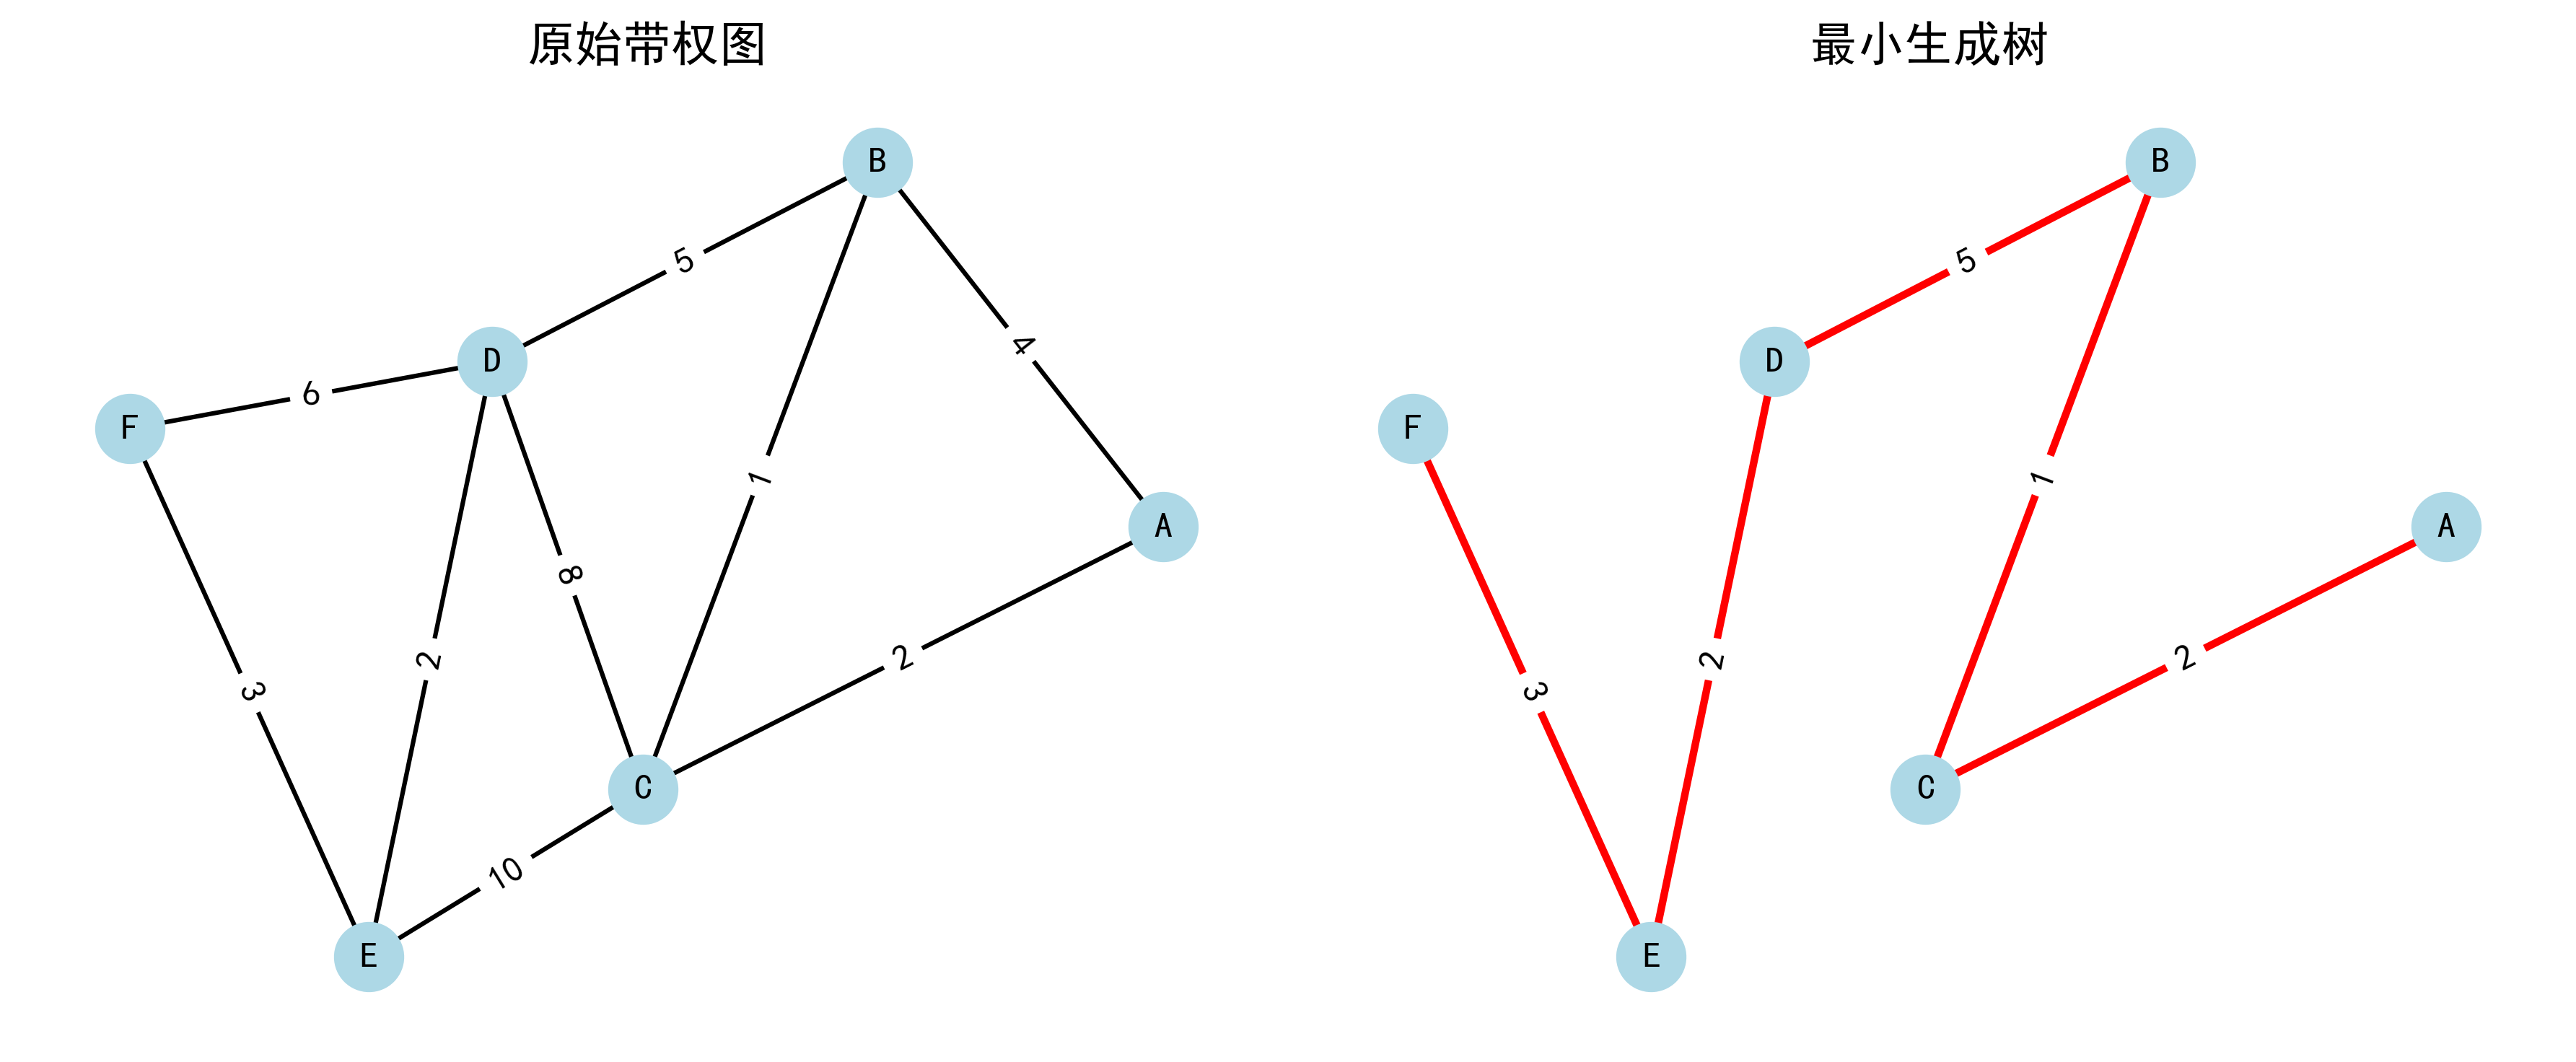
\includegraphics[width=0.9\textwidth]{img/mst_example.png}
    \caption{最小生成树示例:左侧为原图,右侧为最小生成树}
    \label{fig:mst_example}
\end{figure}

\section{最小生成树算法介绍}
\subsection{Prim算法}
Prim算法是一种贪心算法,它从图的任意一个顶点开始,逐步将新的顶点加入到已构建的生成树中,直到所有顶点都被纳入。在每一步中,算法选择一条权重最小的边,这条边连接了已在生成树中的一个顶点和尚未在生成树中的一个顶点。

Prim算法的基本思想是:
\begin{enumerate}
    \item 初始时,生成树中只有一个起始顶点
    \item 在每次迭代中,选择一条连接树中顶点与树外顶点的最小权边,将该边和对应的树外顶点加入到树中
    \item 重复此过程直到所有顶点都被纳入生成树
\end{enumerate}

Prim算法的伪代码如算法\ref{alg:prim}所示。

\begin{algorithm}
    \caption{Prim算法}\label{alg:prim}
    \begin{algorithmic}[1]
    \Procedure{Prim}{$G, w$}\Comment{$G=(V,E)$ 是图,$w$ 是边的权重函数}
    \State $A \gets \emptyset$ \Comment{$A$ 是生成树的边集合,初始为空}
    \State 选择任意一个顶点 $r \in V$ 作为起始顶点
    \State $S \gets \{r\}$ \Comment{$S$ 是已经加入生成树的顶点集合}
    \While{$S \neq V$}\Comment{当还有顶点未加入生成树时}
        \State 选择权重最小的边 $(u,v)$,满足 $u \in S$, $v \in V-S$
        \State $A \gets A \cup \{(u,v)\}$ \Comment{将边 $(u,v)$ 加入生成树}
        \State $S \gets S \cup \{v\}$ \Comment{将顶点 $v$ 加入生成树}
    \EndWhile
    \State \textbf{return} $A$ \Comment{返回最小生成树的边集合}
    \EndProcedure
    \end{algorithmic}
\end{algorithm}

Prim算法可以用不同的数据结构实现,常见的实现有:
\begin{itemize}
    \item \textbf{数组实现}:使用数组存储每个顶点到生成树的最小距离,每次迭代需要 $O(V)$ 时间查找最小距离的顶点,总时间复杂度为 $O(V^2)$
    \item \textbf{优先队列(最小堆)实现}:使用优先队列存储顶点及其到生成树的距离,每次可以在 $O(\log V)$ 时间内找到最小距离的顶点,总时间复杂度为 $O(E \log V)$
\end{itemize}

\subsection{Kruskal算法}
Kruskal算法也是一种贪心算法,但与Prim算法不同,它直接处理图中的边,而不是顶点。算法首先将所有边按权重从小到大排序,然后依次考察每条边,如果该边不会在当前构建的生成树中形成环路,则将其加入生成树。

Kruskal算法的基本思想是:
\begin{enumerate}
    \item 初始时,生成树为空
    \item 将图的所有边按权重从小到大排序
    \item 依次考察每条边,如果添加该边不会形成环路,则将其加入生成树
    \item 重复此过程直到生成树包含 $n-1$ 条边($n$ 是顶点数)
\end{enumerate}

Kruskal算法的伪代码如算法\ref{alg:kruskal}所示。

\begin{algorithm}
    \caption{Kruskal算法}\label{alg:kruskal}
    \begin{algorithmic}[1]
    \Procedure{Kruskal}{$G, w$}\Comment{$G=(V,E)$ 是图,$w$ 是边的权重函数}
    \State $A \gets \emptyset$ \Comment{$A$ 是生成树的边集合,初始为空}
    \For{每个顶点 $v \in V$}
        \State $\textrm{MakeSet}(v)$ \Comment{初始化,每个顶点形成一个单独的集合}
    \EndFor
    \State 将 $E$ 中的所有边按照权重 $w$ 从小到大排序
    \For{每条边 $(u,v) \in E$,按权重从小到大顺序}
        \If{$\textrm{FindSet}(u) \neq \textrm{FindSet}(v)$} \Comment{检查边是否会形成环}
            \State $A \gets A \cup \{(u,v)\}$ \Comment{将边 $(u,v)$ 加入生成树}
            \State $\textrm{Union}(u, v)$ \Comment{合并 $u$ 和 $v$ 所在的集合}
        \EndIf
    \EndFor
    \State \textbf{return} $A$ \Comment{返回最小生成树的边集合}
    \EndProcedure
    \end{algorithmic}
\end{algorithm}

Kruskal算法中的环路检测和集合合并可以用不同的数据结构实现:
\begin{itemize}
    \item \textbf{数组实现}:使用数组记录每个顶点所属的连通分量,但合并操作需要 $O(V)$ 时间,总时间复杂度为 $O(E \times V + E \log E)$
    \item \textbf{并查集实现}:使用并查集(带路径压缩和按秩合并的优化)可以实现近乎常数时间的查找和合并操作,总时间复杂度为 $O(E \log V)$,主要受限于边的排序
\end{itemize}

\section{算法实现与比较}
本节将通过实验比较Prim算法和Kruskal算法在不同实现和不同图类型上的性能表现。实验使用C++实现了五种不同的最小生成树算法:
\begin{itemize}
    \item Prim算法(数组实现,使用邻接矩阵)
    \item Prim算法(优先队列实现,使用邻接矩阵)
    \item Prim算法(优先队列实现,使用邻接表 - 优化版)
    \item Kruskal算法(数组实现)
    \item Kruskal算法(并查集实现)
\end{itemize}

实验通过随机生成不同规模的图,比较了这些算法在稀疏图和稠密图上的运行时间,每组实验运行多次取平均值以确保结果的可靠性。实验使用了节点数为50到500的图,对于稀疏图使用0.05的边概率,对于稠密图使用0.9的边概率。每种配置运行5次并取平均值,以减少随机波动对结果的影响。为了确保实验的可重复性,所有随机生成的图都保证了连通性,并使用相同的随机种子。

\subsection{算法性能提升}
\subsubsection{Prim算法的数据结构优化}
图\ref{fig:prim_sparse}和图\ref{fig:prim_dense}分别展示了Prim算法在稀疏图和稠密图上使用不同数据结构实现的性能比较。

\begin{figure}[htbp]
    \centering
    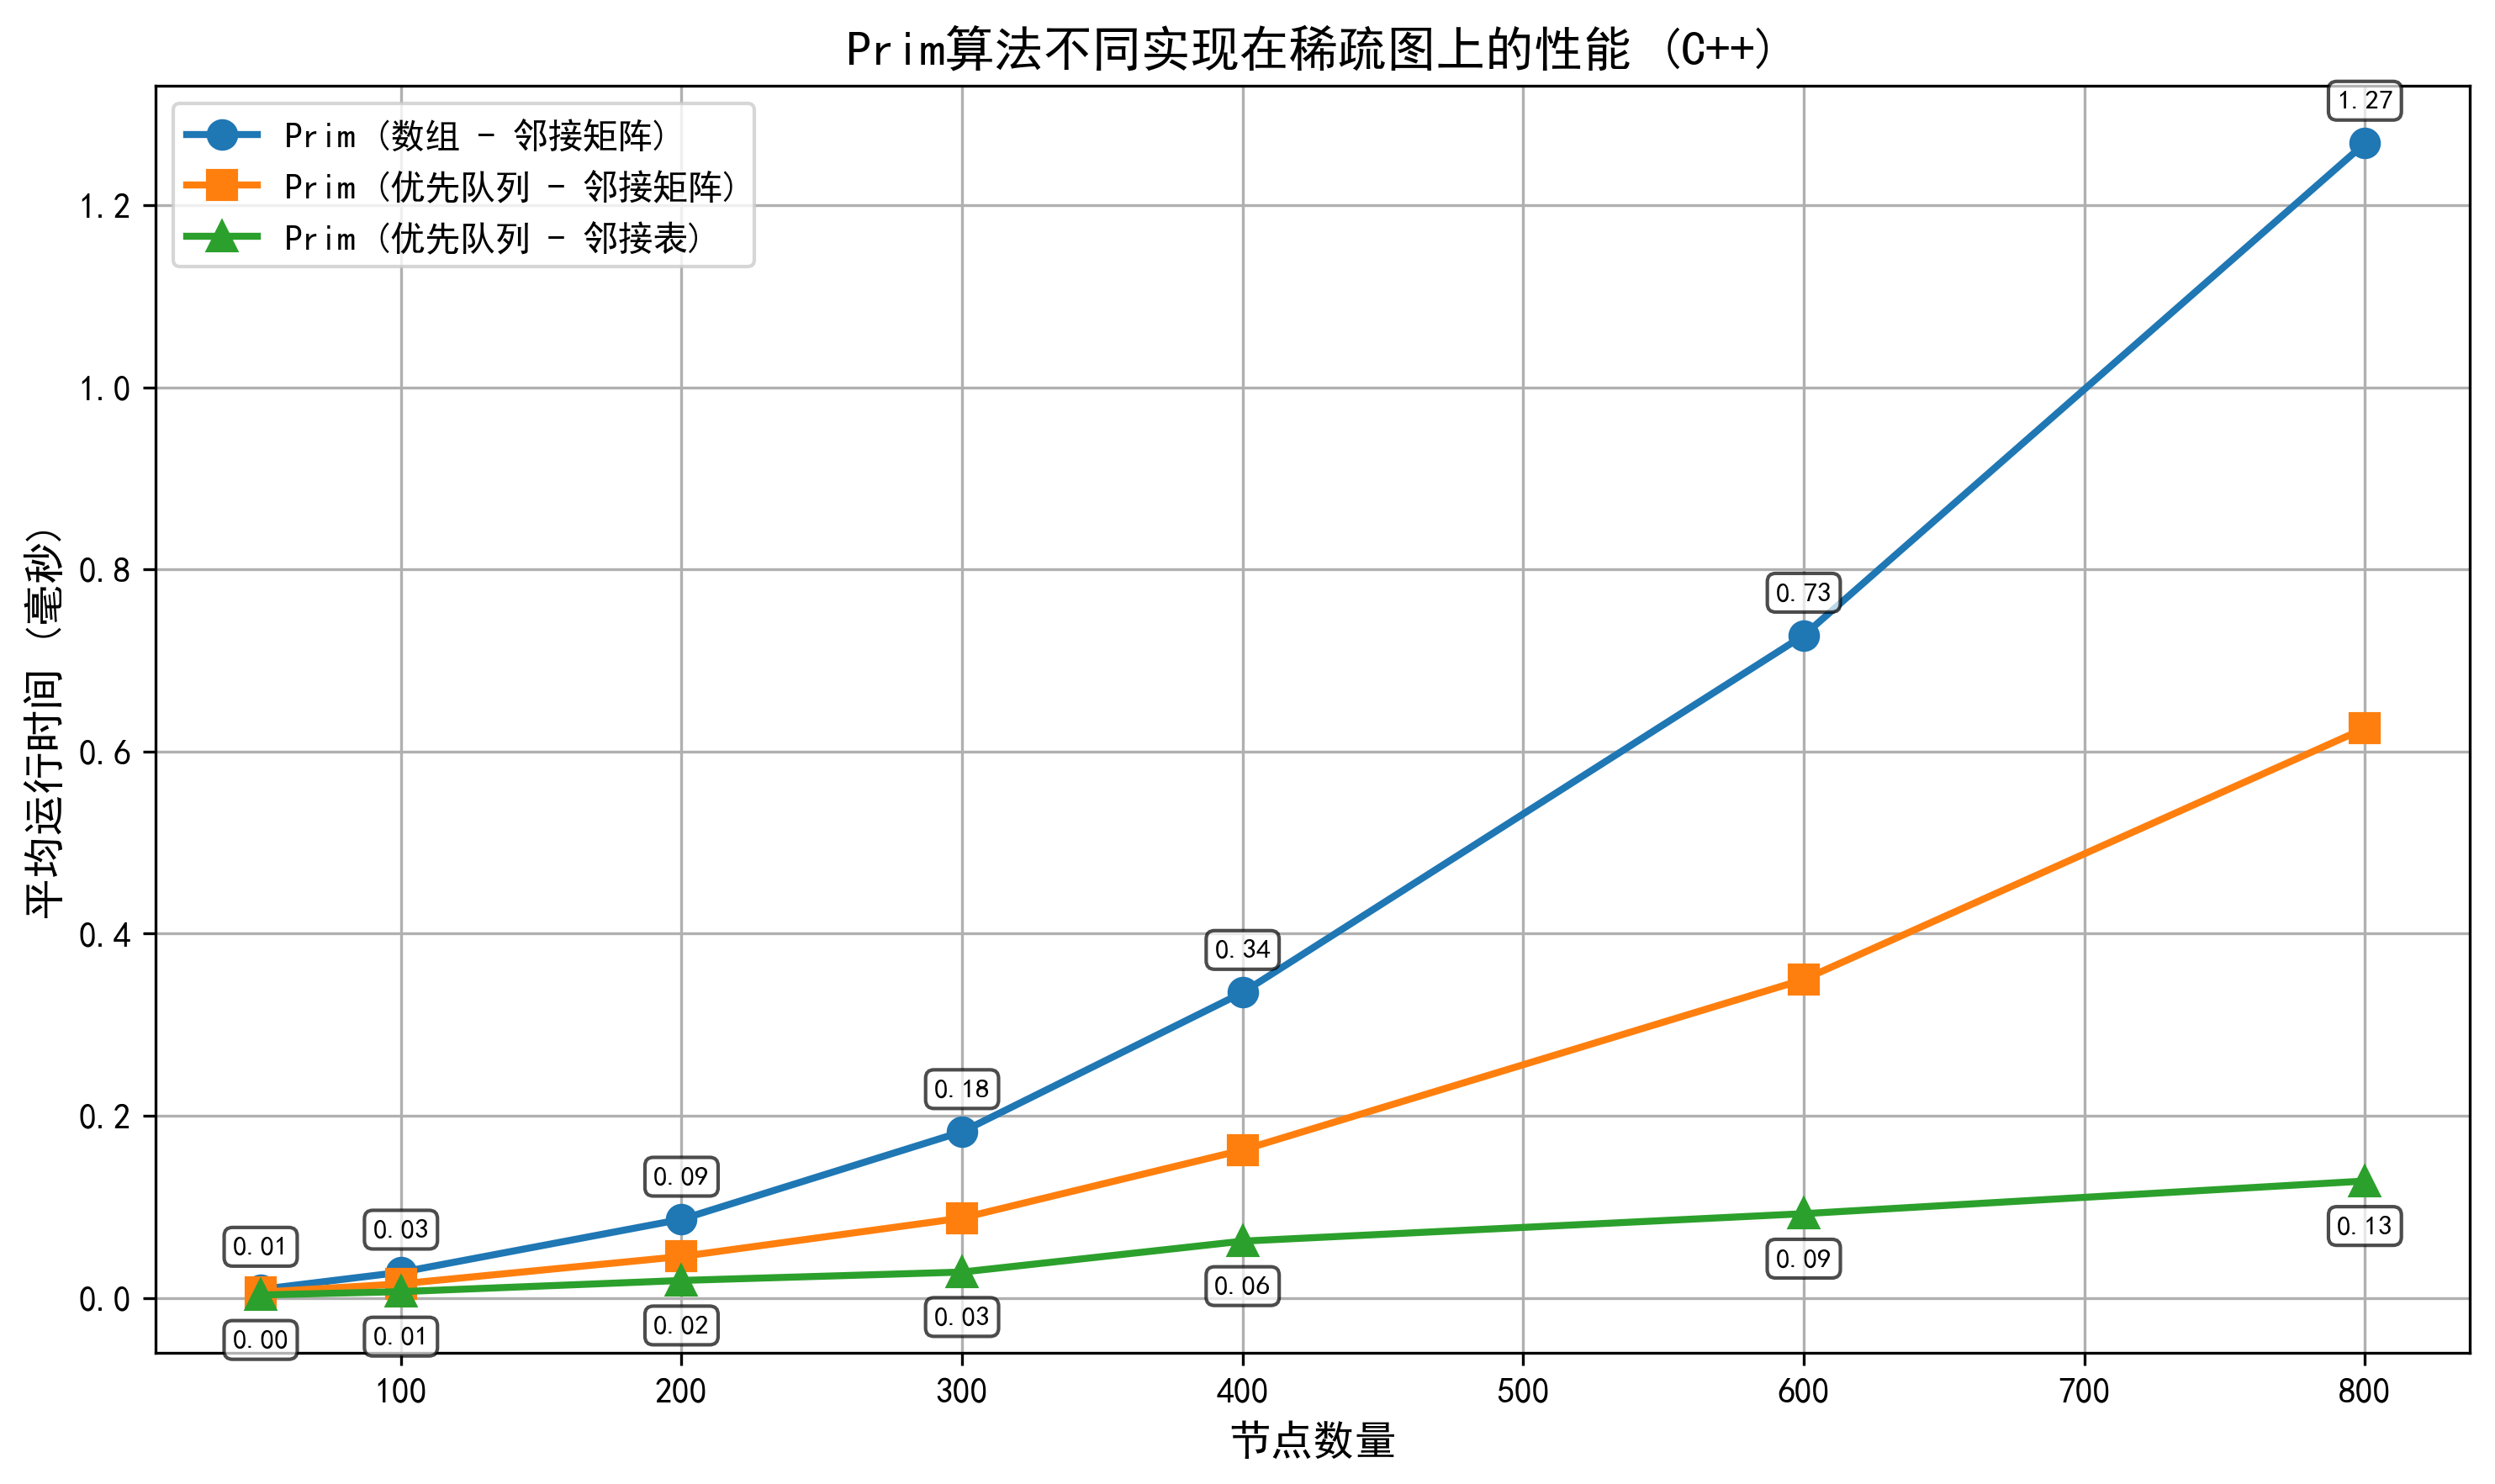
\includegraphics[width=0.8\textwidth]{img/img_cpp2/prim_sparse_comparison_cpp.png}
    \caption{Prim算法在稀疏图上的性能比较}
    \label{fig:prim_sparse}
\end{figure}

\begin{figure}[htbp]
    \centering
    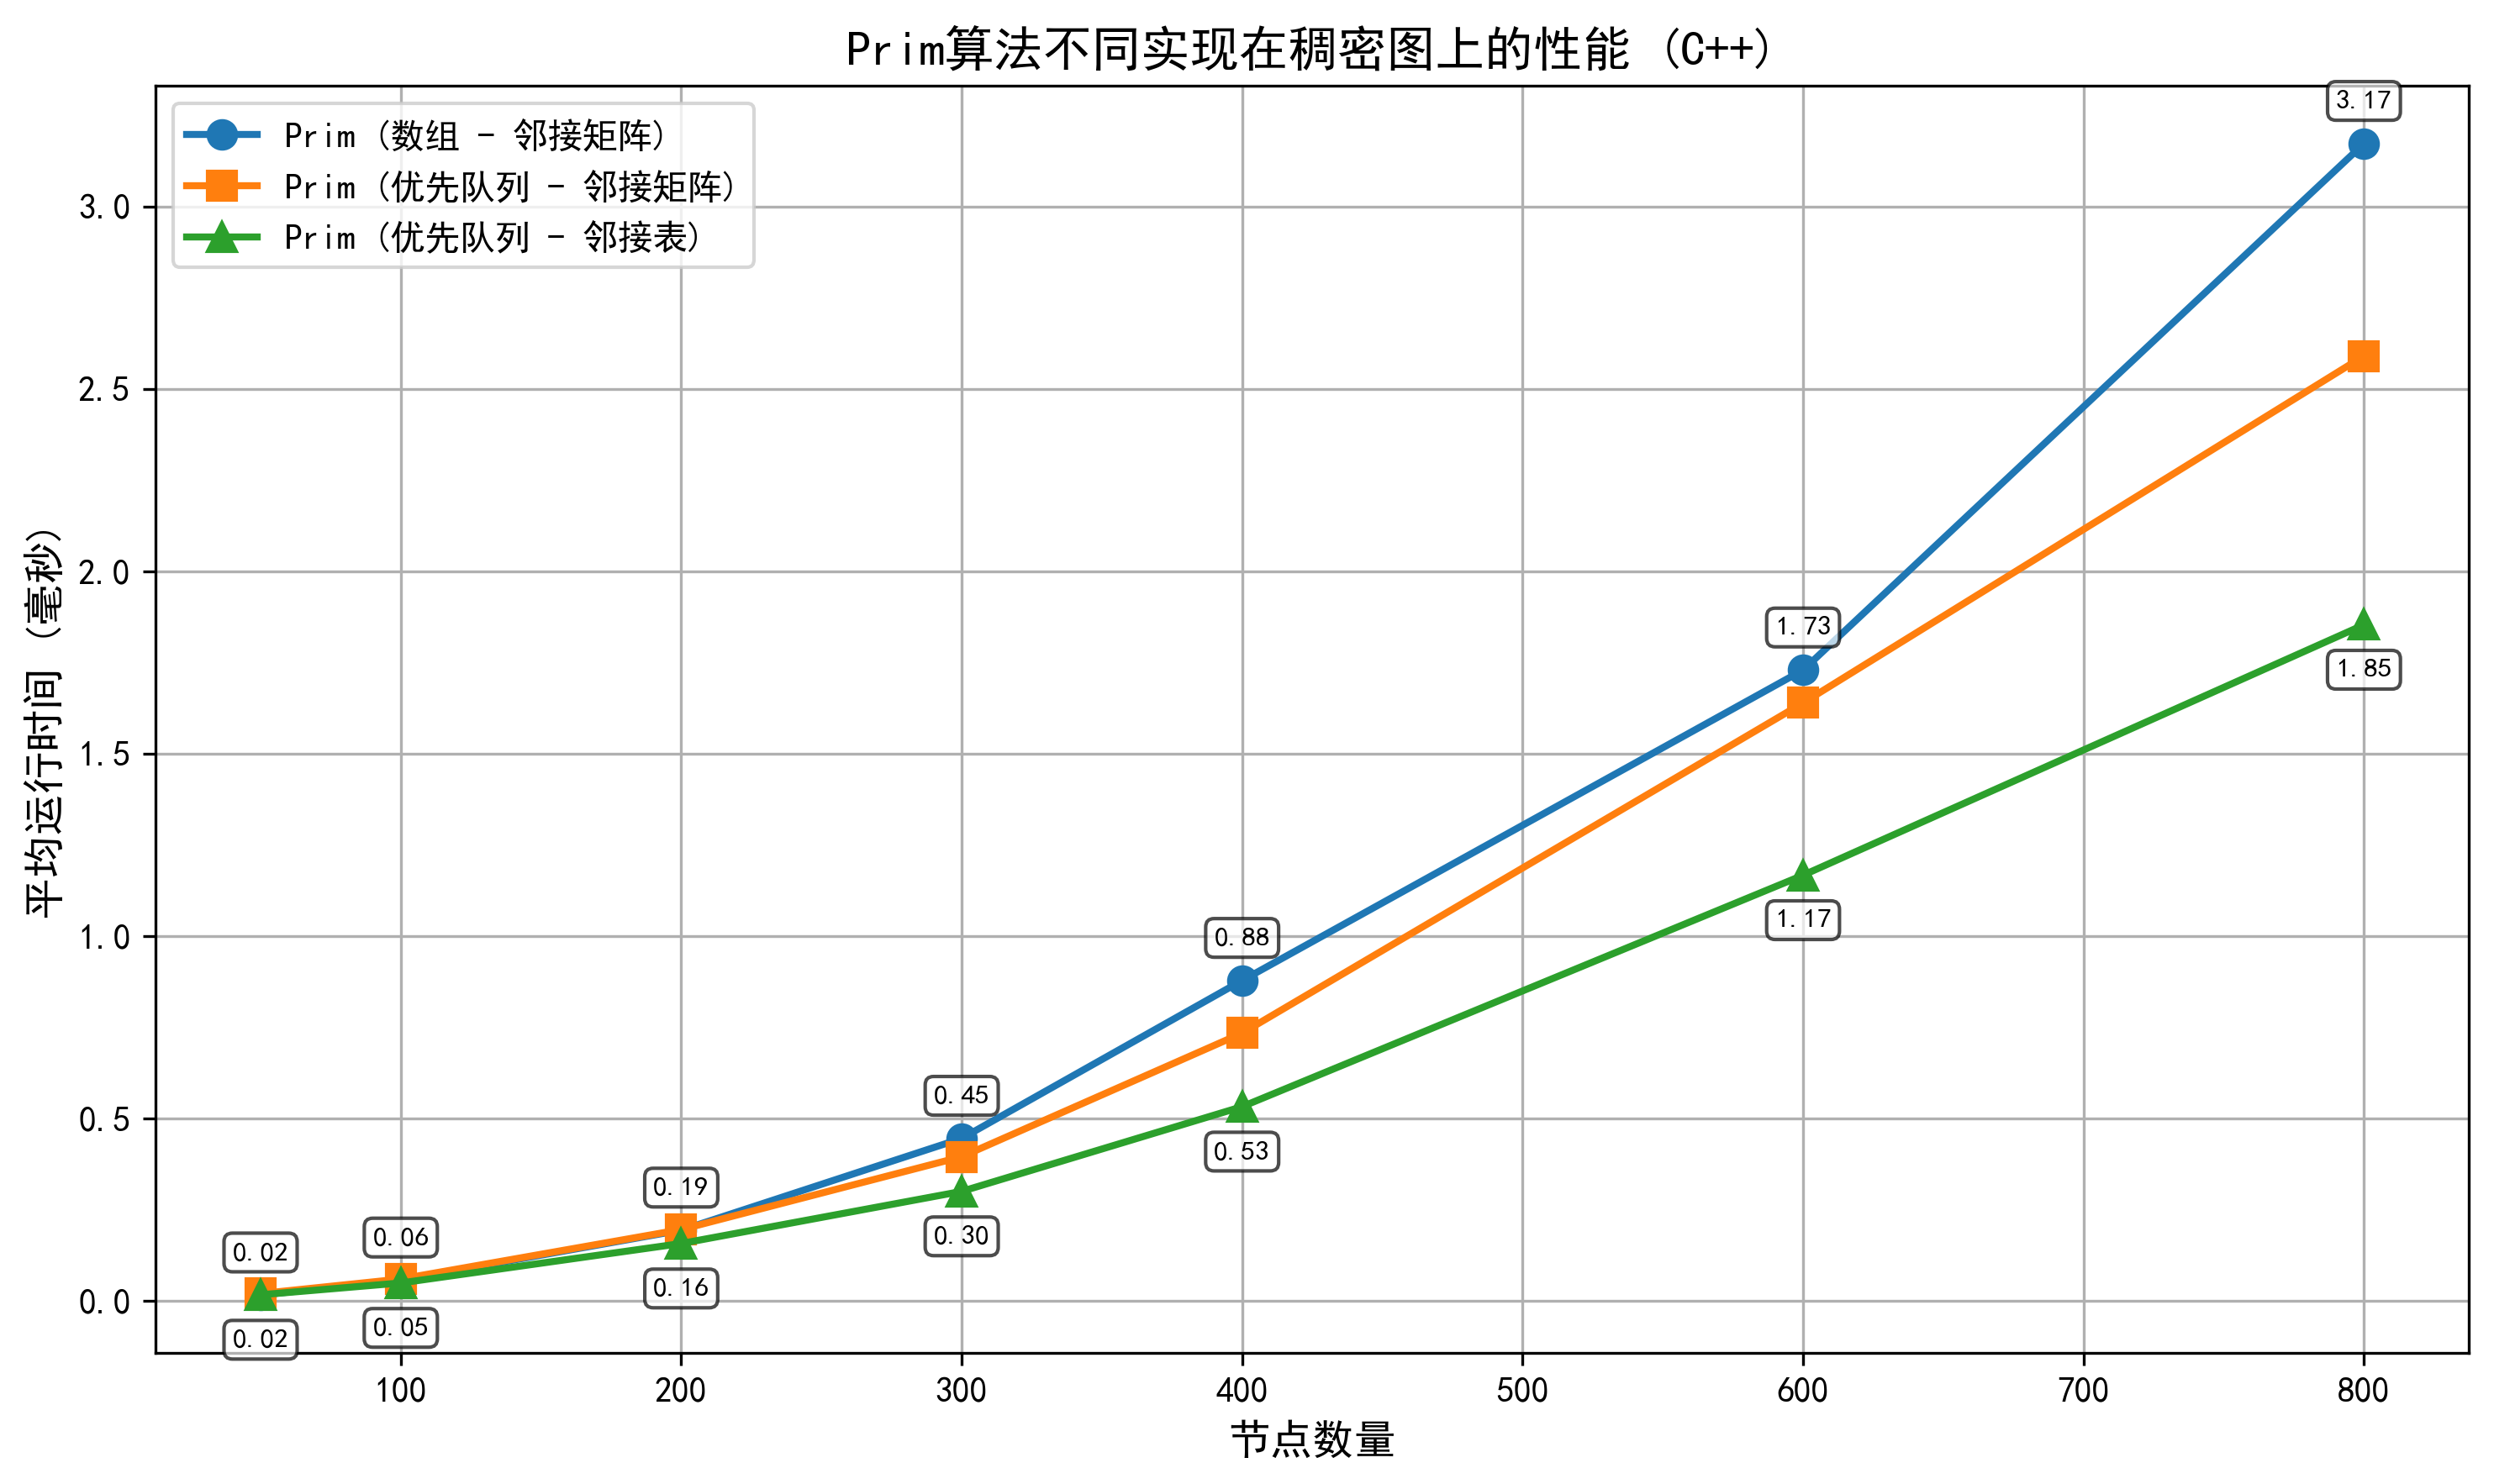
\includegraphics[width=0.8\textwidth]{img/img_cpp2/prim_dense_comparison_cpp.png}
    \caption{Prim算法在稠密图上的性能比较}
    \label{fig:prim_dense}
\end{figure}

根据实验结果可以得出:
\begin{itemize}
    \item 在稀疏图上,优先队列实现(特别是优先队列+邻接表实现)的Prim算法明显优于数组实现,随着节点数增加,性能差距更加明显
    \item 在稠密图上,所有实现的性能差异相对较小,但优先队列+邻接表实现仍然表现最佳    
\end{itemize}

这一现象可以从理论上解释:
\begin{itemize}
    \item 数组实现的Prim算法时间复杂度为 $O(V^2)$,不依赖于边的数量
    \item 优先队列+邻接矩阵实现的Prim算法时间复杂度为 $O(E \log V + V^2)$,因为需要初始化邻接矩阵
    \item 优先队列+邻接表实现的Prim算法时间复杂度为 $O(E \log V)$
    \item 在稀疏图中,$E \approx V$,此时 $O(E \log V) \approx O(V \log V)$,明显优于 $O(V^2)$
    \item 在稠密图中,$E \approx V^2$,此时邻接表的优势不如稀疏图明显
\end{itemize}

\subsubsection{Kruskal算法的数据结构优化}
图\ref{fig:kruskal_sparse}和图\ref{fig:kruskal_dense}分别展示了Kruskal算法在稀疏图和稠密图上使用不同数据结构实现的性能比较。为了更直观地理解这些算法的工作原理,可以参考算法可视化工具\cite{prim_visual},它提供了交互式的最小生成树算法演示。

\begin{figure}[htbp]
    \centering
    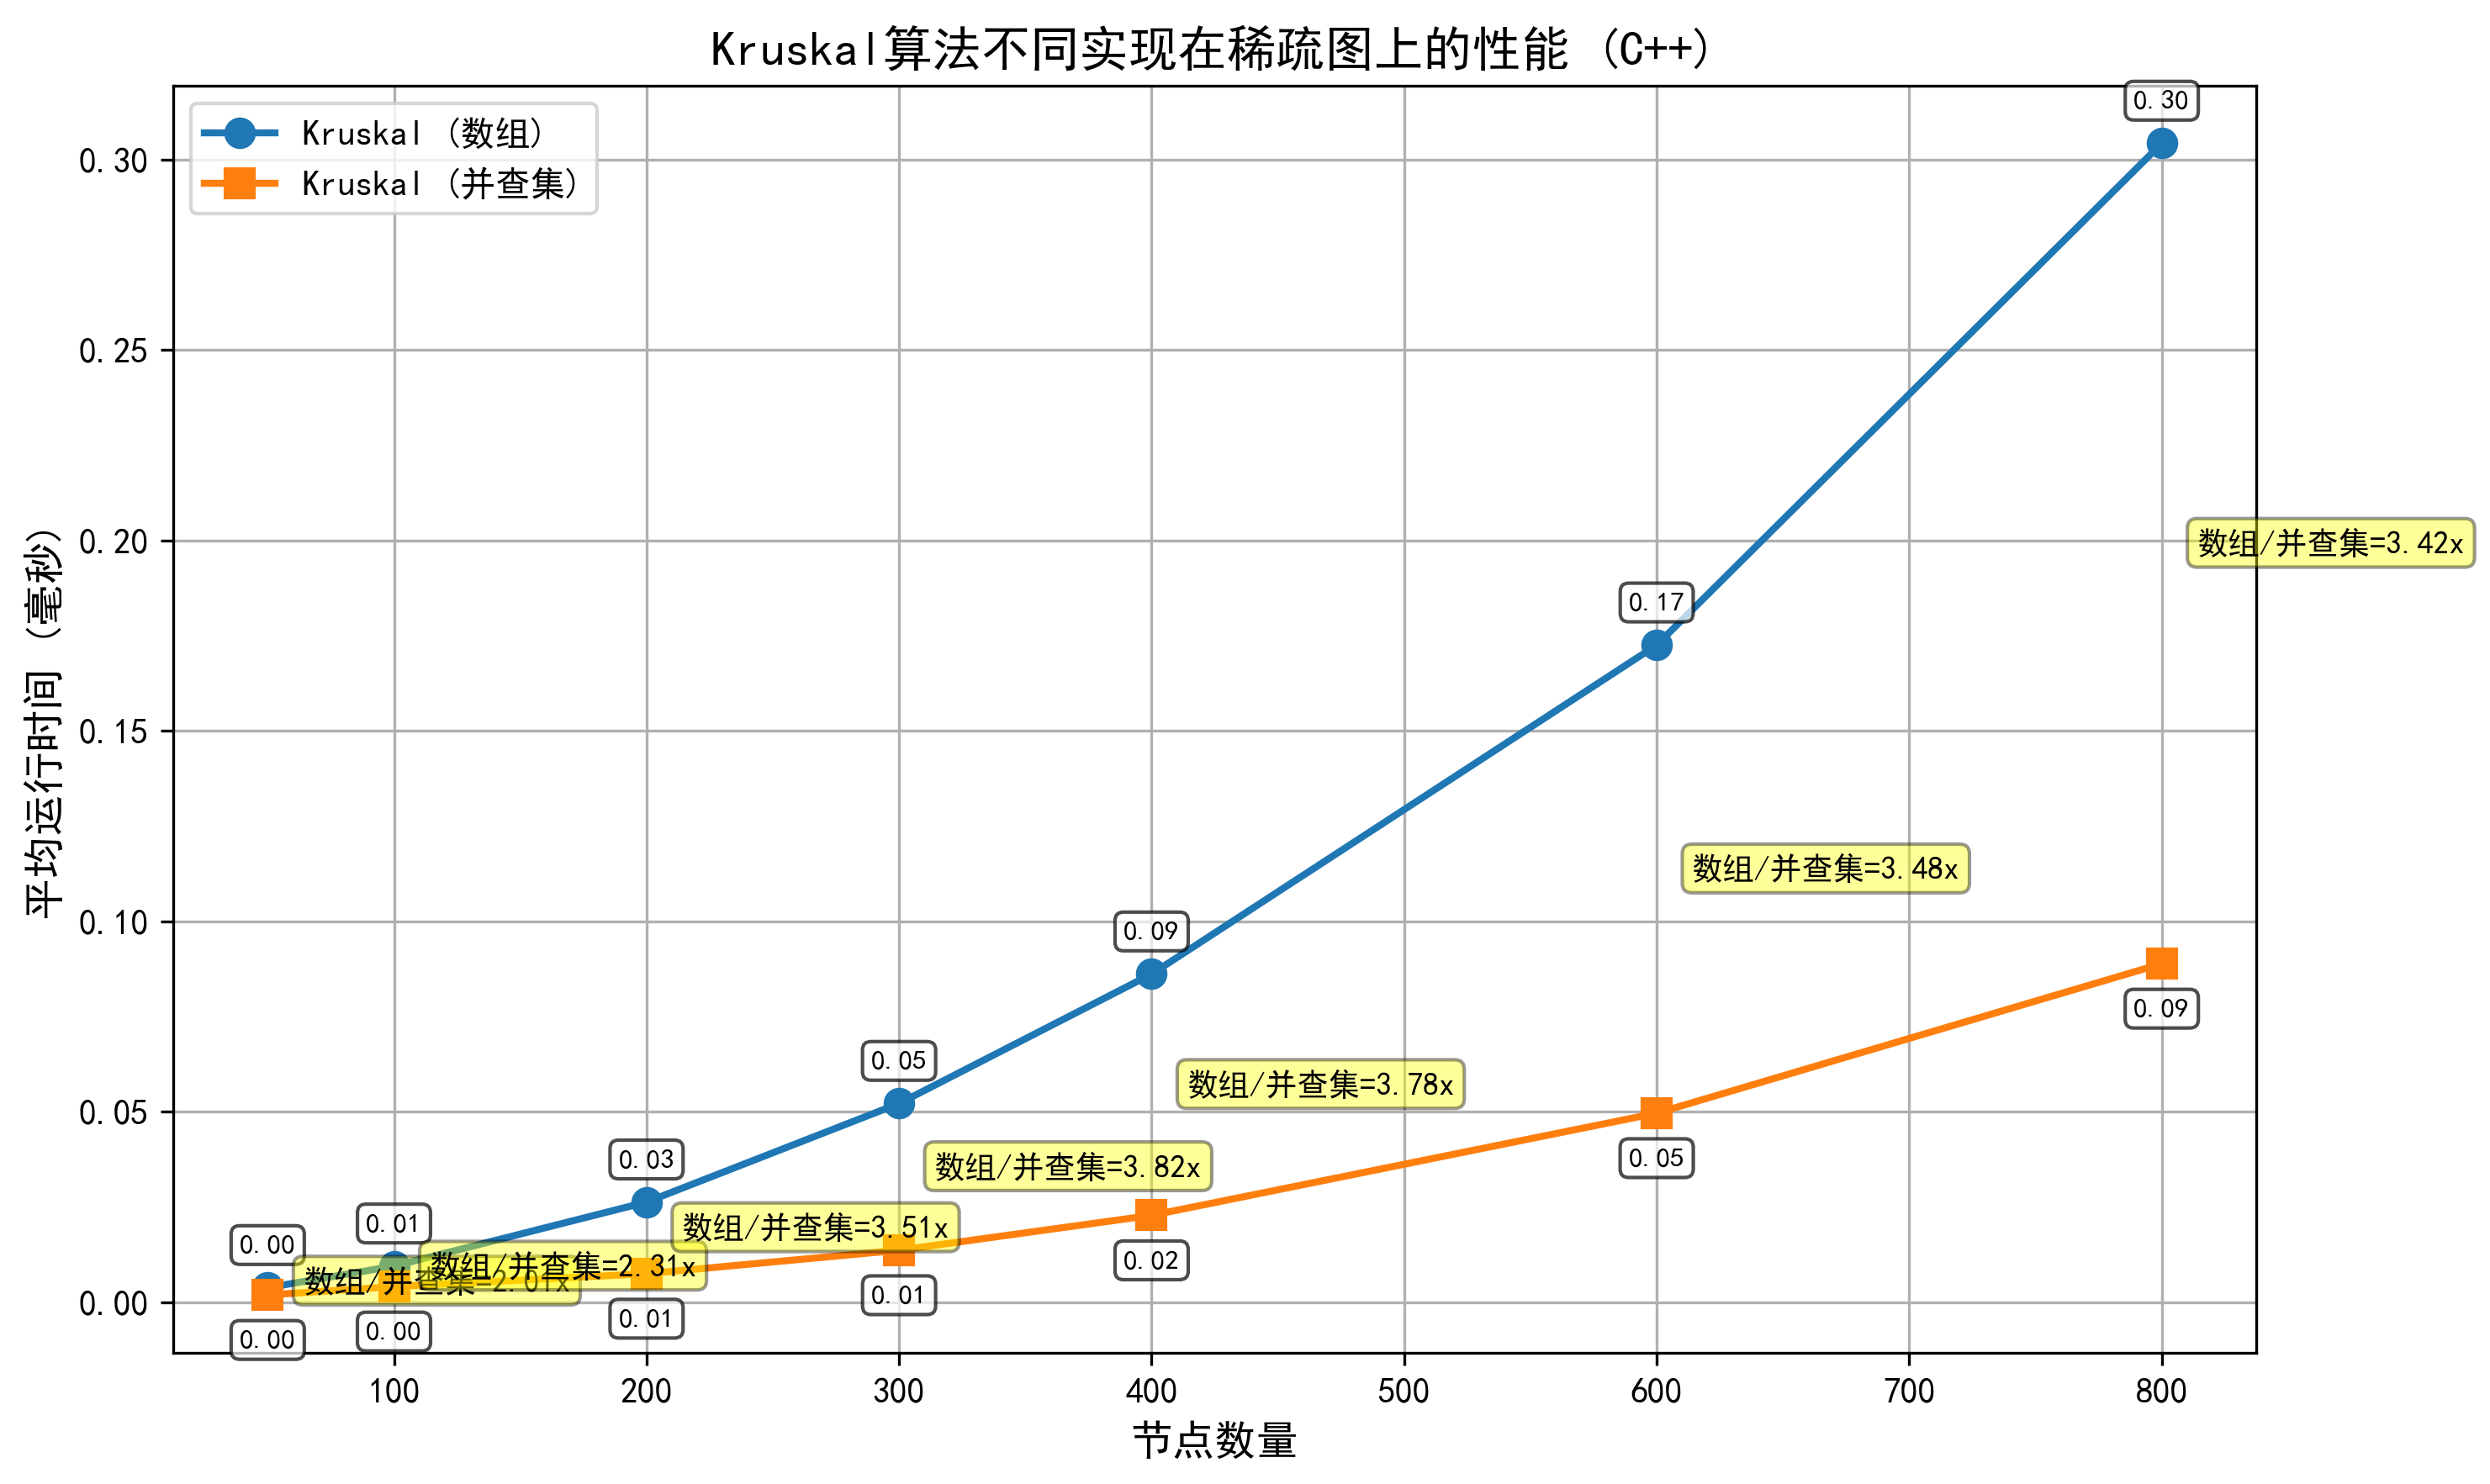
\includegraphics[width=0.8\textwidth]{img/img_cpp2/kruskal_sparse_comparison_cpp.png}
    \caption{Kruskal算法在稀疏图上的性能比较}
    \label{fig:kruskal_sparse}
\end{figure}

\begin{figure}[htbp]
    \centering
    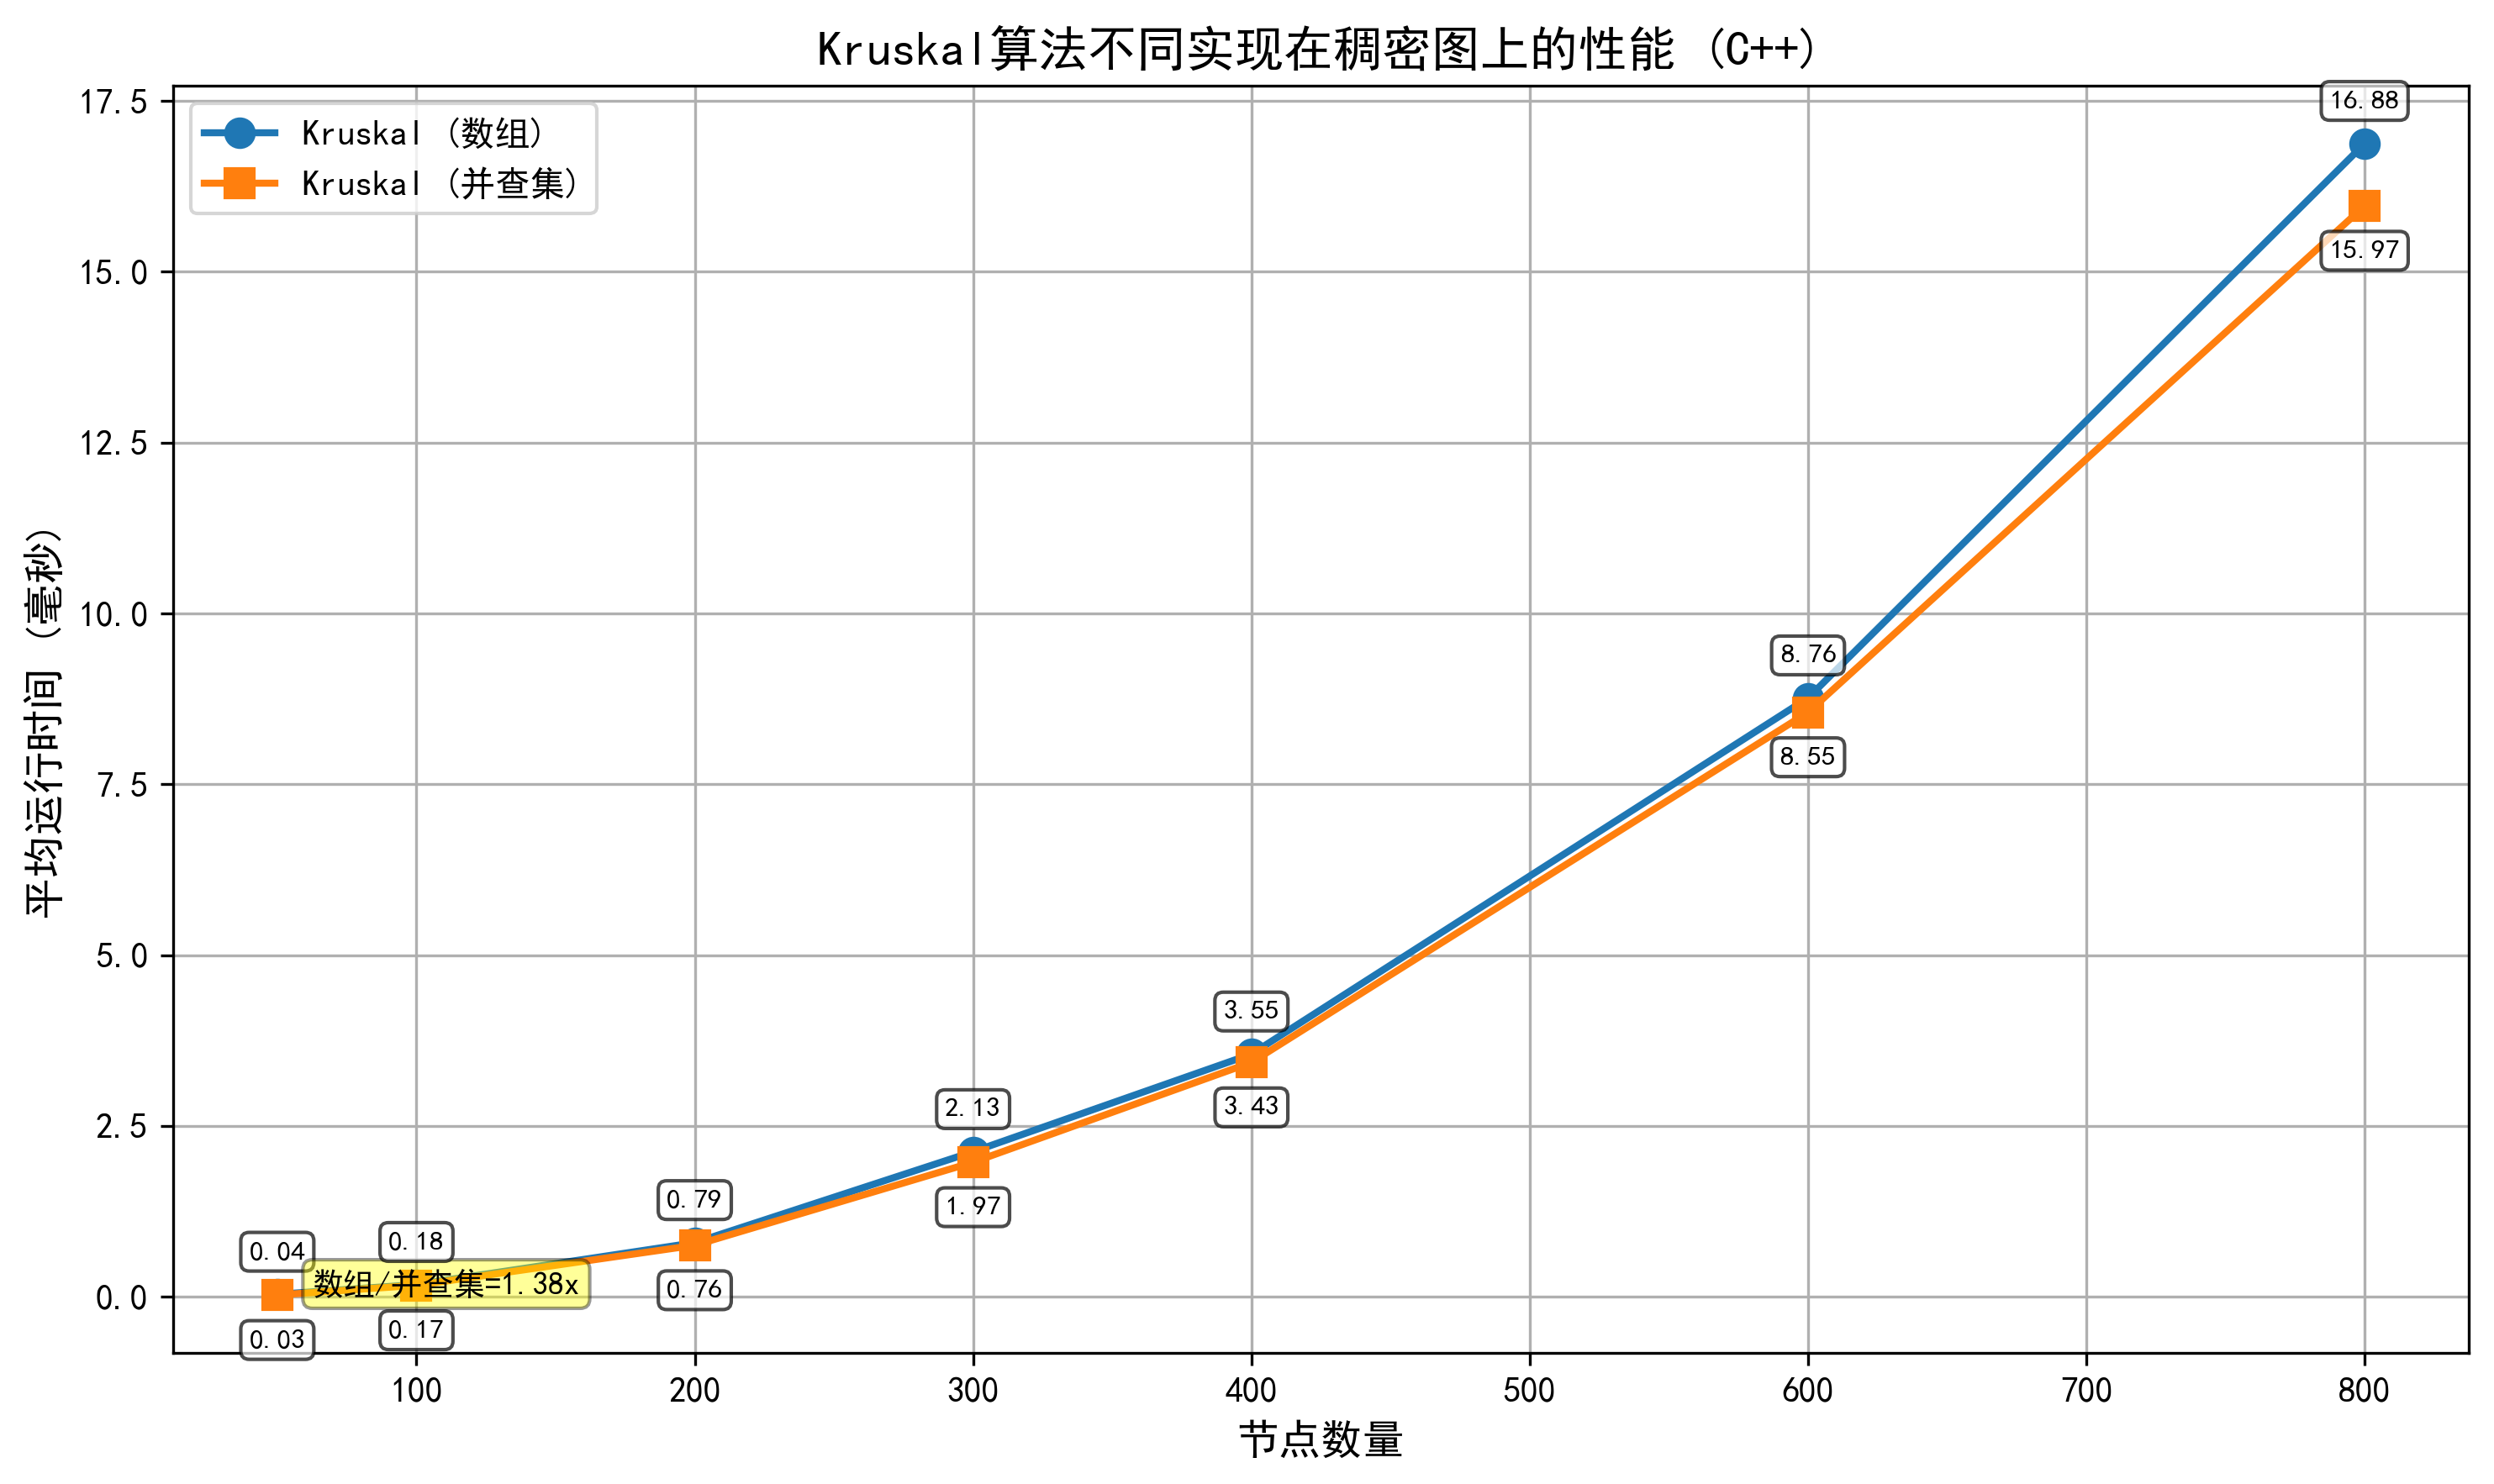
\includegraphics[width=0.8\textwidth]{img/img_cpp2/kruskal_dense_comparison_cpp.png}
    \caption{Kruskal算法在稠密图上的性能比较}
    \label{fig:kruskal_dense}
\end{figure}

从图中可以观察到:
\begin{itemize}
    \item 在稀疏图上,并查集实现的Kruskal算法明显优于数组实现,差距随着图规模增加而更明显
    \item 在稠密图上,两种实现的性能差距相对较小,尤其在大规模图上几乎相当
    \item 在稠密图上,两种实现的性能都显著下降,这是因为边的数量增加导致排序和处理时间增加
\end{itemize}

从理论上分析:
\begin{itemize}
    \item 数组实现的Kruskal算法时间复杂度为 $O(E \log E + E \times V)$,其中 $E \log E$ 来自于边的排序,$E \times V$ 来自于每次合并操作需要 $O(V)$ 时间
    \item 并查集实现的Kruskal算法时间复杂度为 $O(E \log E + E \times \alpha(V))$,其中 $\alpha(V)$ 是阿克曼函数的反函数,在实际应用中几乎是常数
    \item 在稠密图中($E \approx V^2$),排序的 $O(E \log E)$ 部分成为主导因素,占据了算法的大部分运行时间
    \item 当排序成为主要瓶颈时,合并操作(无论是数组还是并查集实现)的时间差异在总运行时间中的占比变得相对较小
\end{itemize}

这一现象的理论解释可能是:
\begin{itemize}
    \item \textbf{排序开销主导}:在稠密图中,边数量为 $O(V^2)$,排序这些边的开销 $O(V^2 \log V^2)$ 远大于后续处理的开销,使得不同数据结构在合并操作上的差异变得不那么显著
    \item \textbf{内存局部性影响}:在处理大量边时,排序算法的缓存局部性可能成为性能瓶颈,掩盖了并查集和数组实现在合并操作上的差异。关于内存访问模式对算法性能的影响,Drepper的研究\cite{cache_locality}提供了深入的分析。
    \item \textbf{实际操作次数}:在最小生成树算法中,即使图很稠密,最终加入MST的边数仍然只有 $V-1$ 条,因此实际执行的合并操作数量有限,减小了两种实现的差异
\end{itemize}

\subsection{算法适用场景分析}
图\ref{fig:optimal_sparse}和图\ref{fig:optimal_dense}比较了最优实现的Prim算法(优先队列+邻接表实现)和Kruskal算法(并查集实现)在稀疏图和稠密图上的性能。

\begin{figure}[htbp]
    \centering
    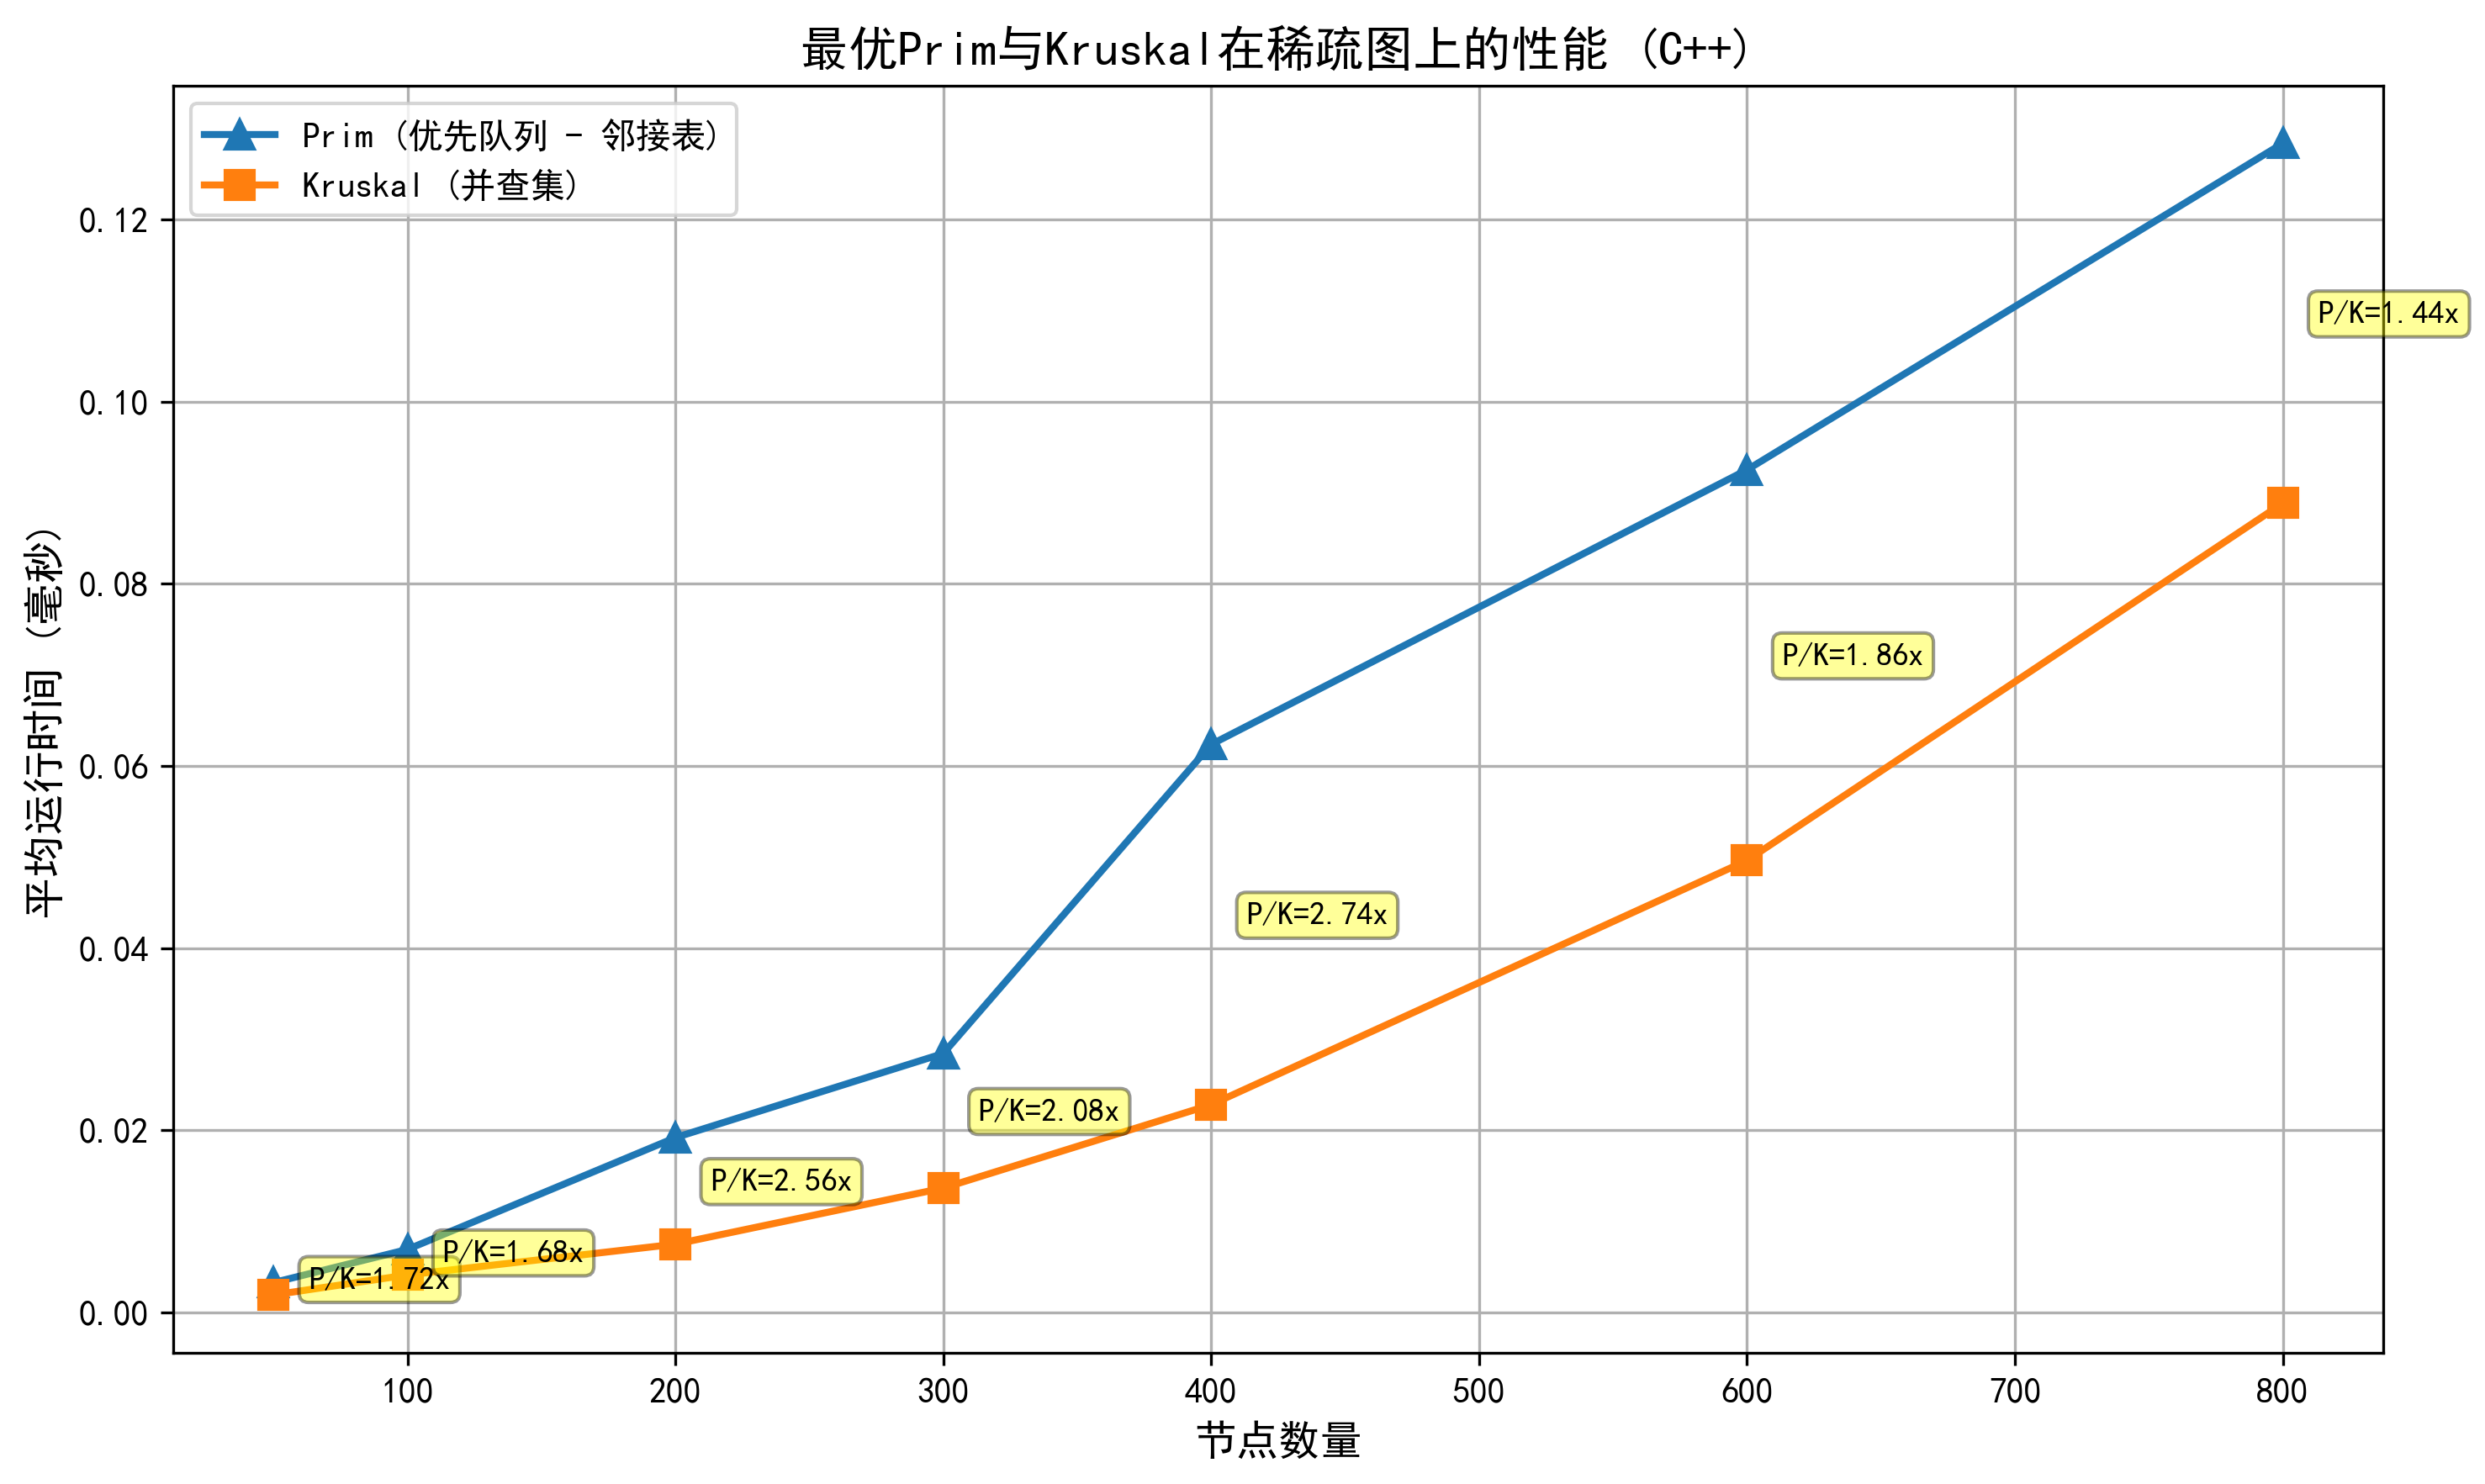
\includegraphics[width=0.8\textwidth]{img/img_cpp2/optimal_sparse_comparison_cpp.png}
    \caption{最优实现的Prim与Kruskal算法在稀疏图上的性能比较}
    \label{fig:optimal_sparse}
\end{figure}

\begin{figure}[htbp]
    \centering
    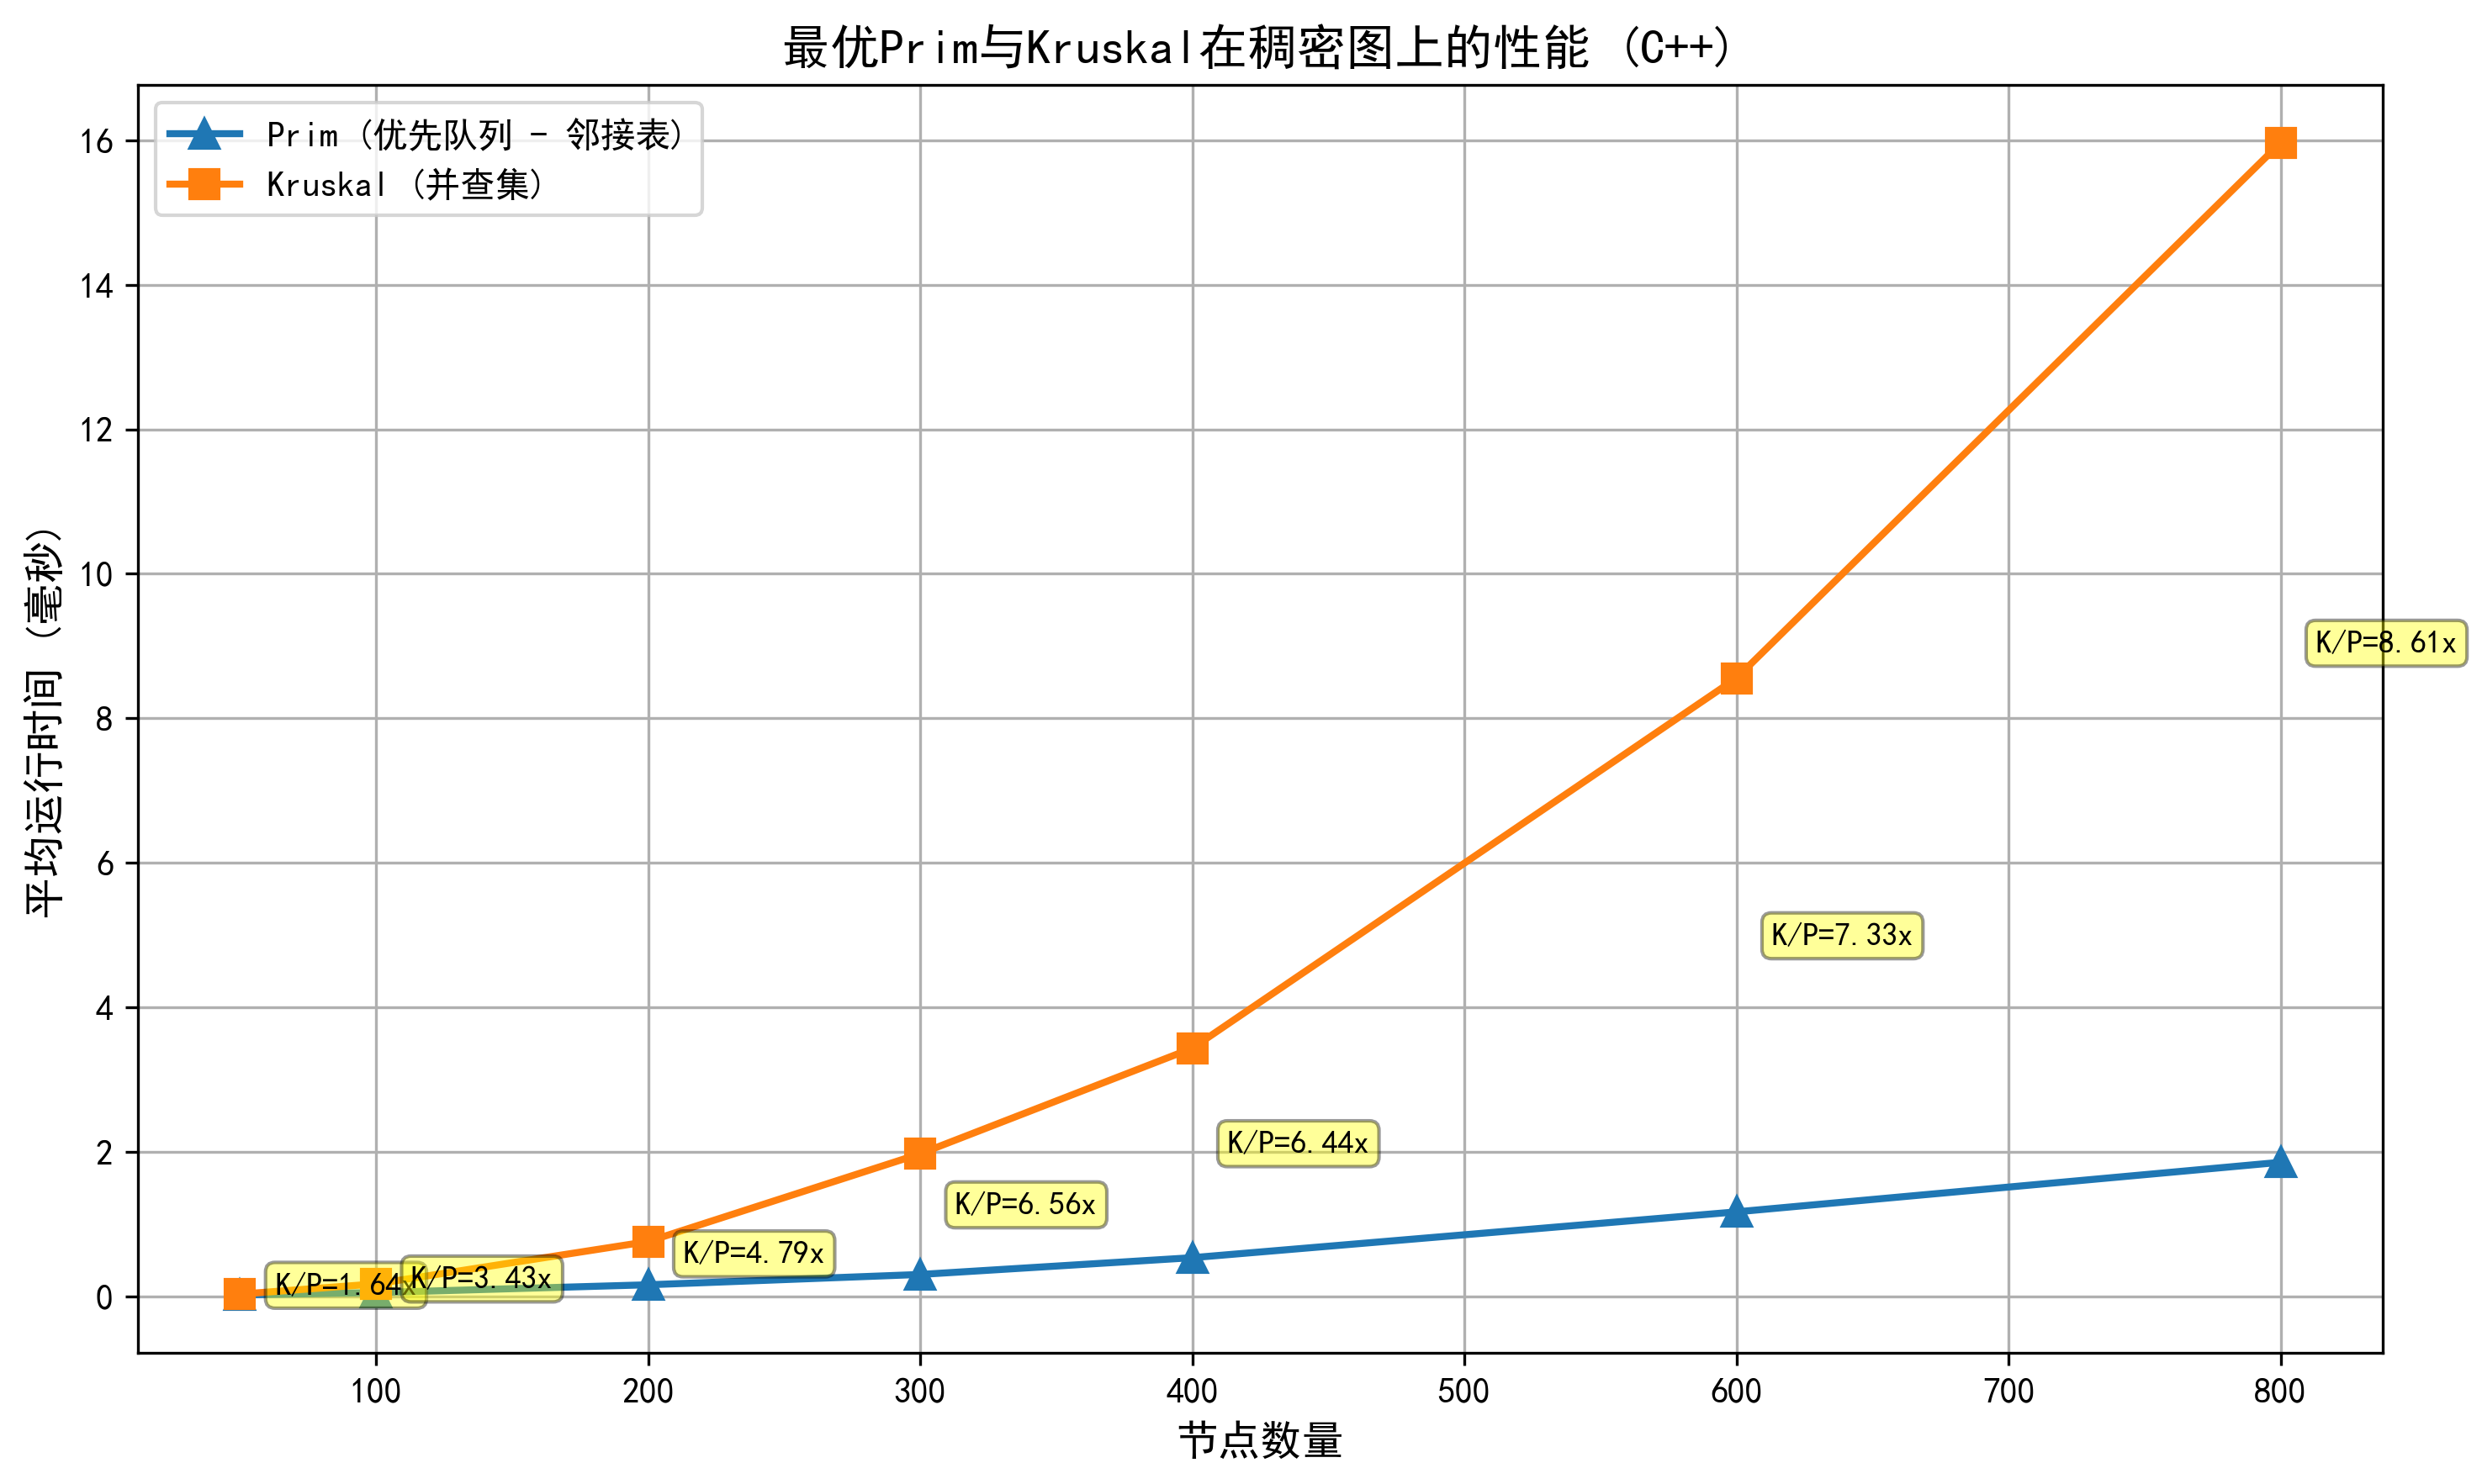
\includegraphics[width=0.8\textwidth]{img/img_cpp2/optimal_dense_comparison_cpp.png}
    \caption{最优实现的Prim与Kruskal算法在稠密图上的性能比较}
    \label{fig:optimal_dense}
\end{figure}

\begin{figure}[htbp]
    \centering
    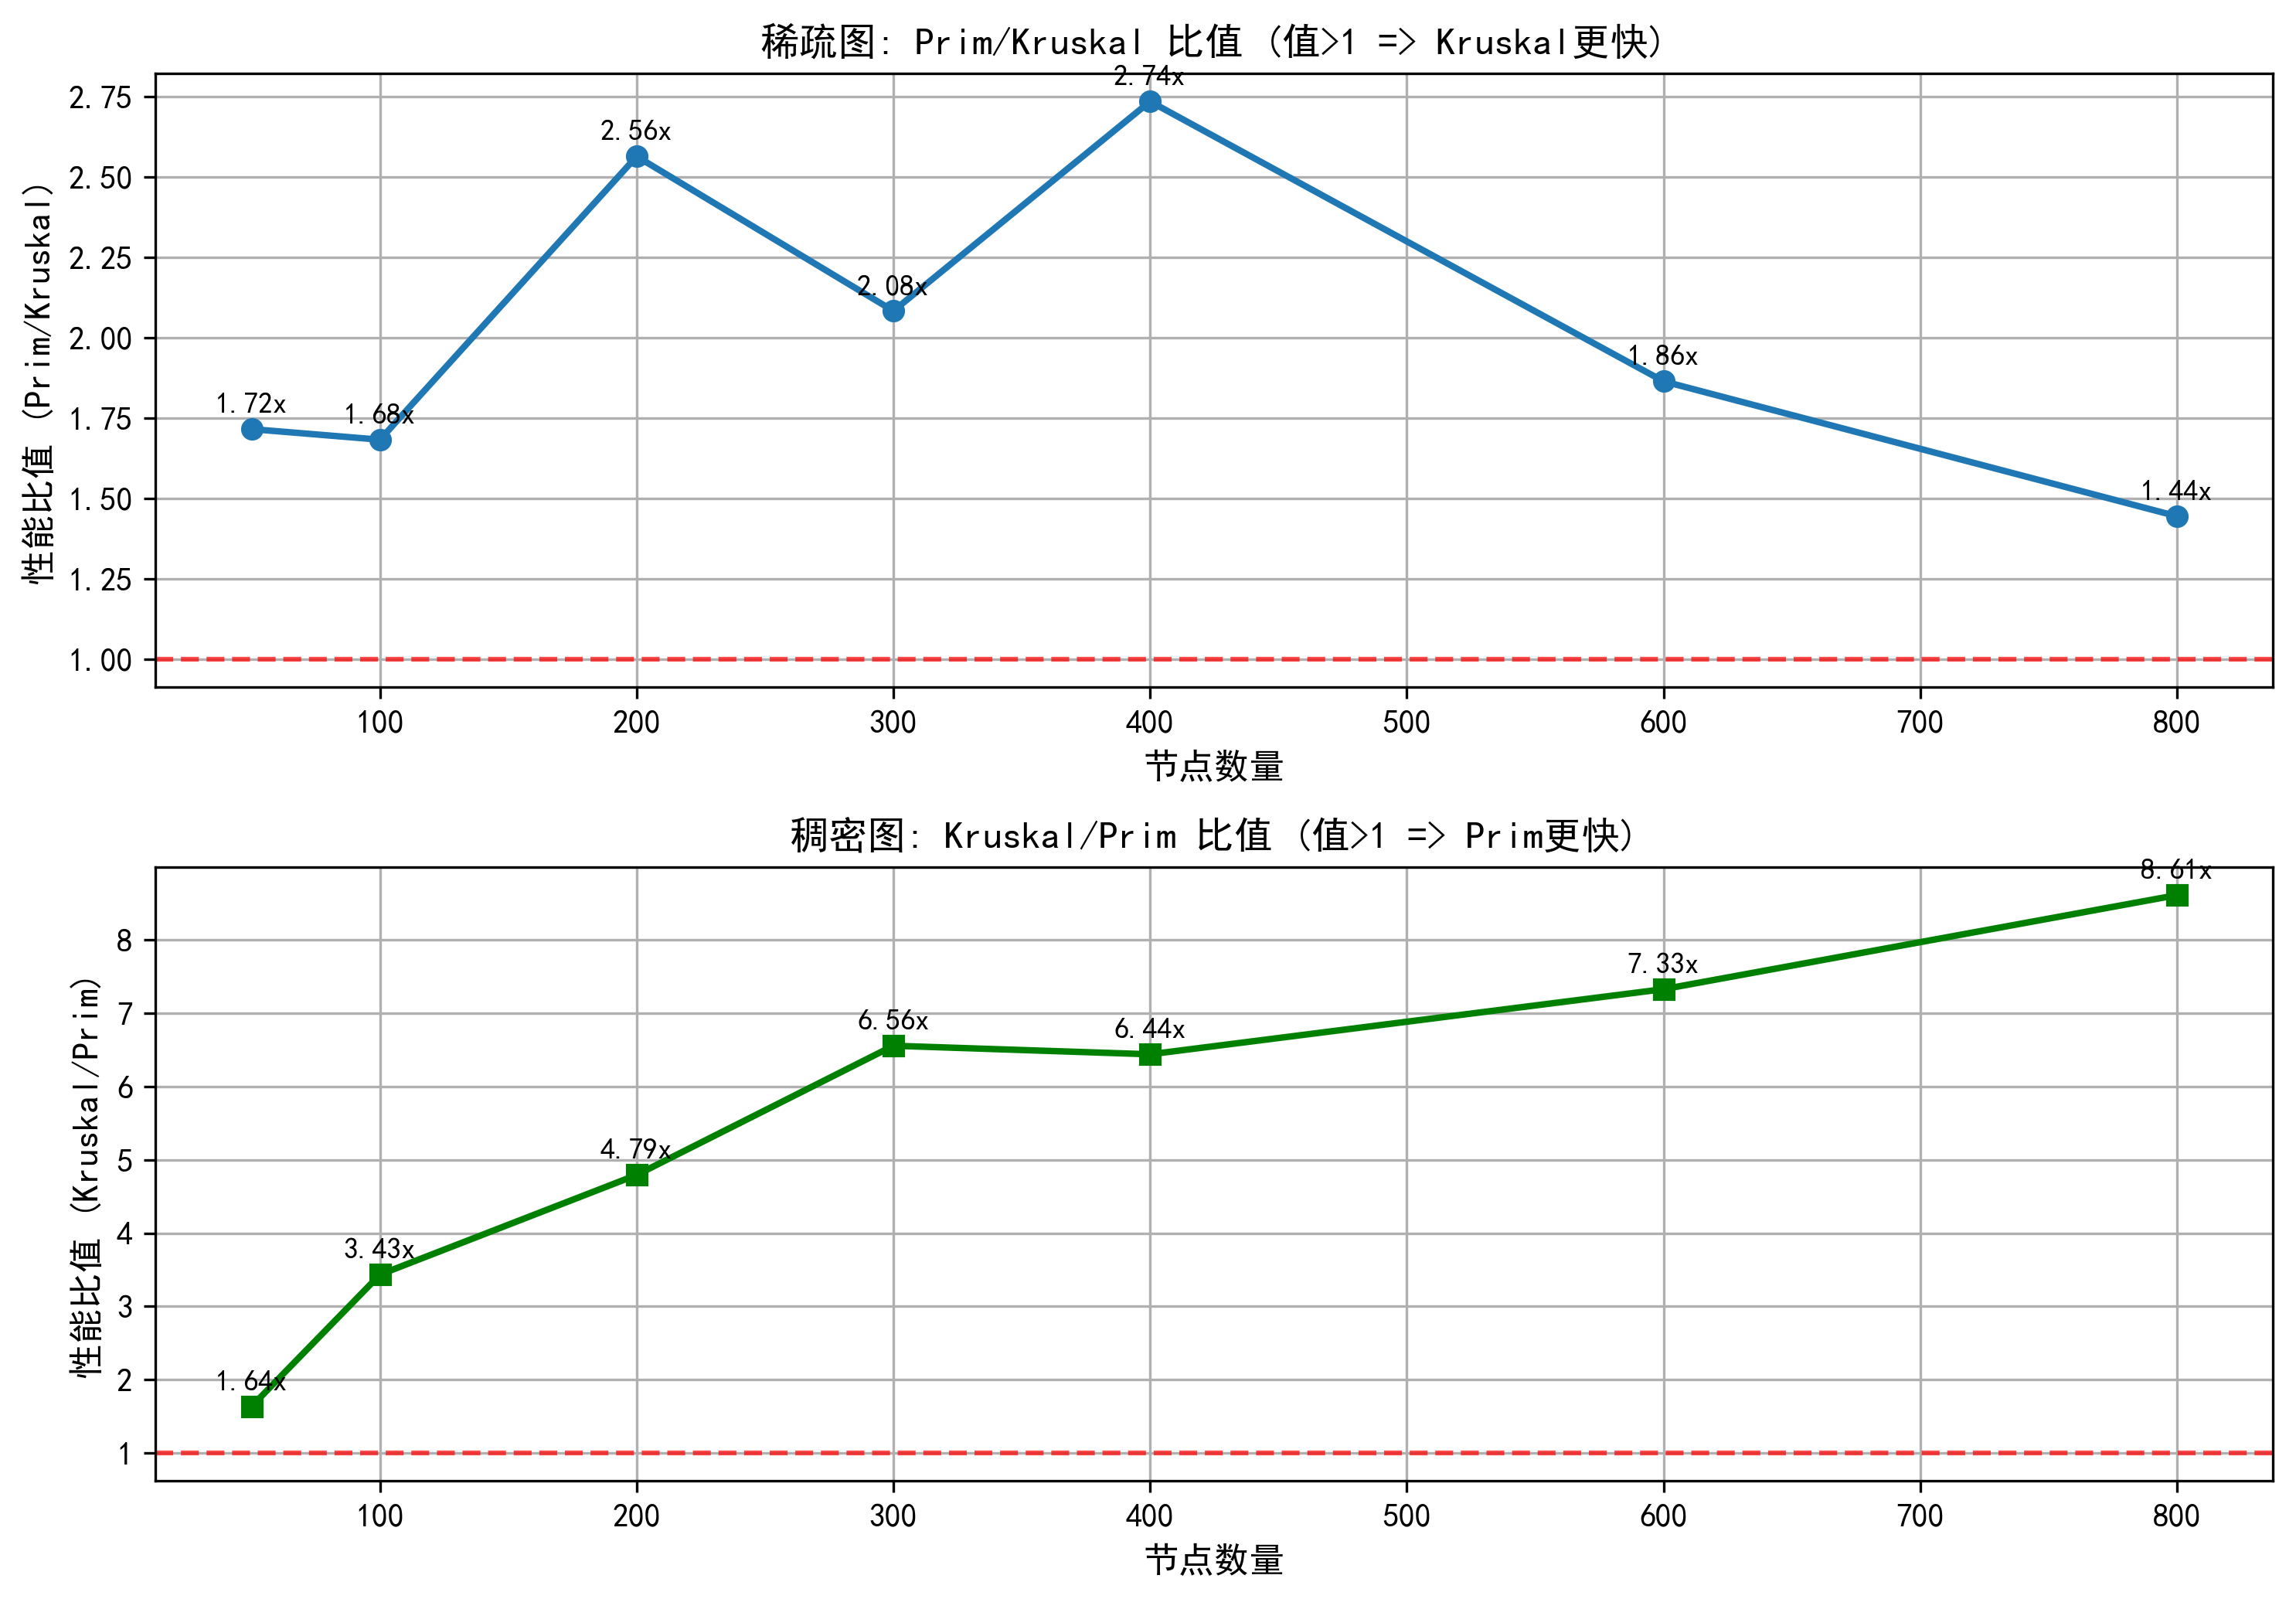
\includegraphics[width=0.8\textwidth]{img/img_cpp2/theory_vs_actual_cpp.png}
    \caption{最优实现的Prim与Kruskal算法性能比值}
    \label{fig:optimal_dense}
\end{figure}

预期理论分析:
\begin{itemize}
    \item 优先队列+邻接表实现的Prim算法时间复杂度为 $O(E \log V)$
    \item 并查集实现的Kruskal算法时间复杂度为 $O(E \log E) \approx O(E \log V)$(因为 $E \leq V^2$,所以 $\log E \leq 2\log V$)
    \item 在稀疏图中($E \approx V$),Kruskal算法的排序开销较小,而且只需要处理较少的边
    \item 在稠密图中($E \approx V^2$),Kruskal算法需要排序和处理大量边($O(V^2 \log V^2)$),而Prim算法虽然也需要处理所有边,但优先队列操作次数与节点数相关($O(V^2 \log V)$),理论上更有优势
\end{itemize}

实际实验测试:
\begin{itemize}
    \item 在稠密图上,Prim算法(优先队列+邻接表实现)明显优于Kruskal算法(并查集实现),随着节点数增加,性能差距越来越大
    \item 然而,在稀疏图上,在图规模较小时,Kruskal算法(并查集实现)通常比Prim算法(优先队列+邻接表实现)性能更好
    \item 但当图规模增加到一定量级时,Prim算法的效率会反超Kruskal算法。
\end{itemize}

\begin{figure}[htbp]
    \centering
    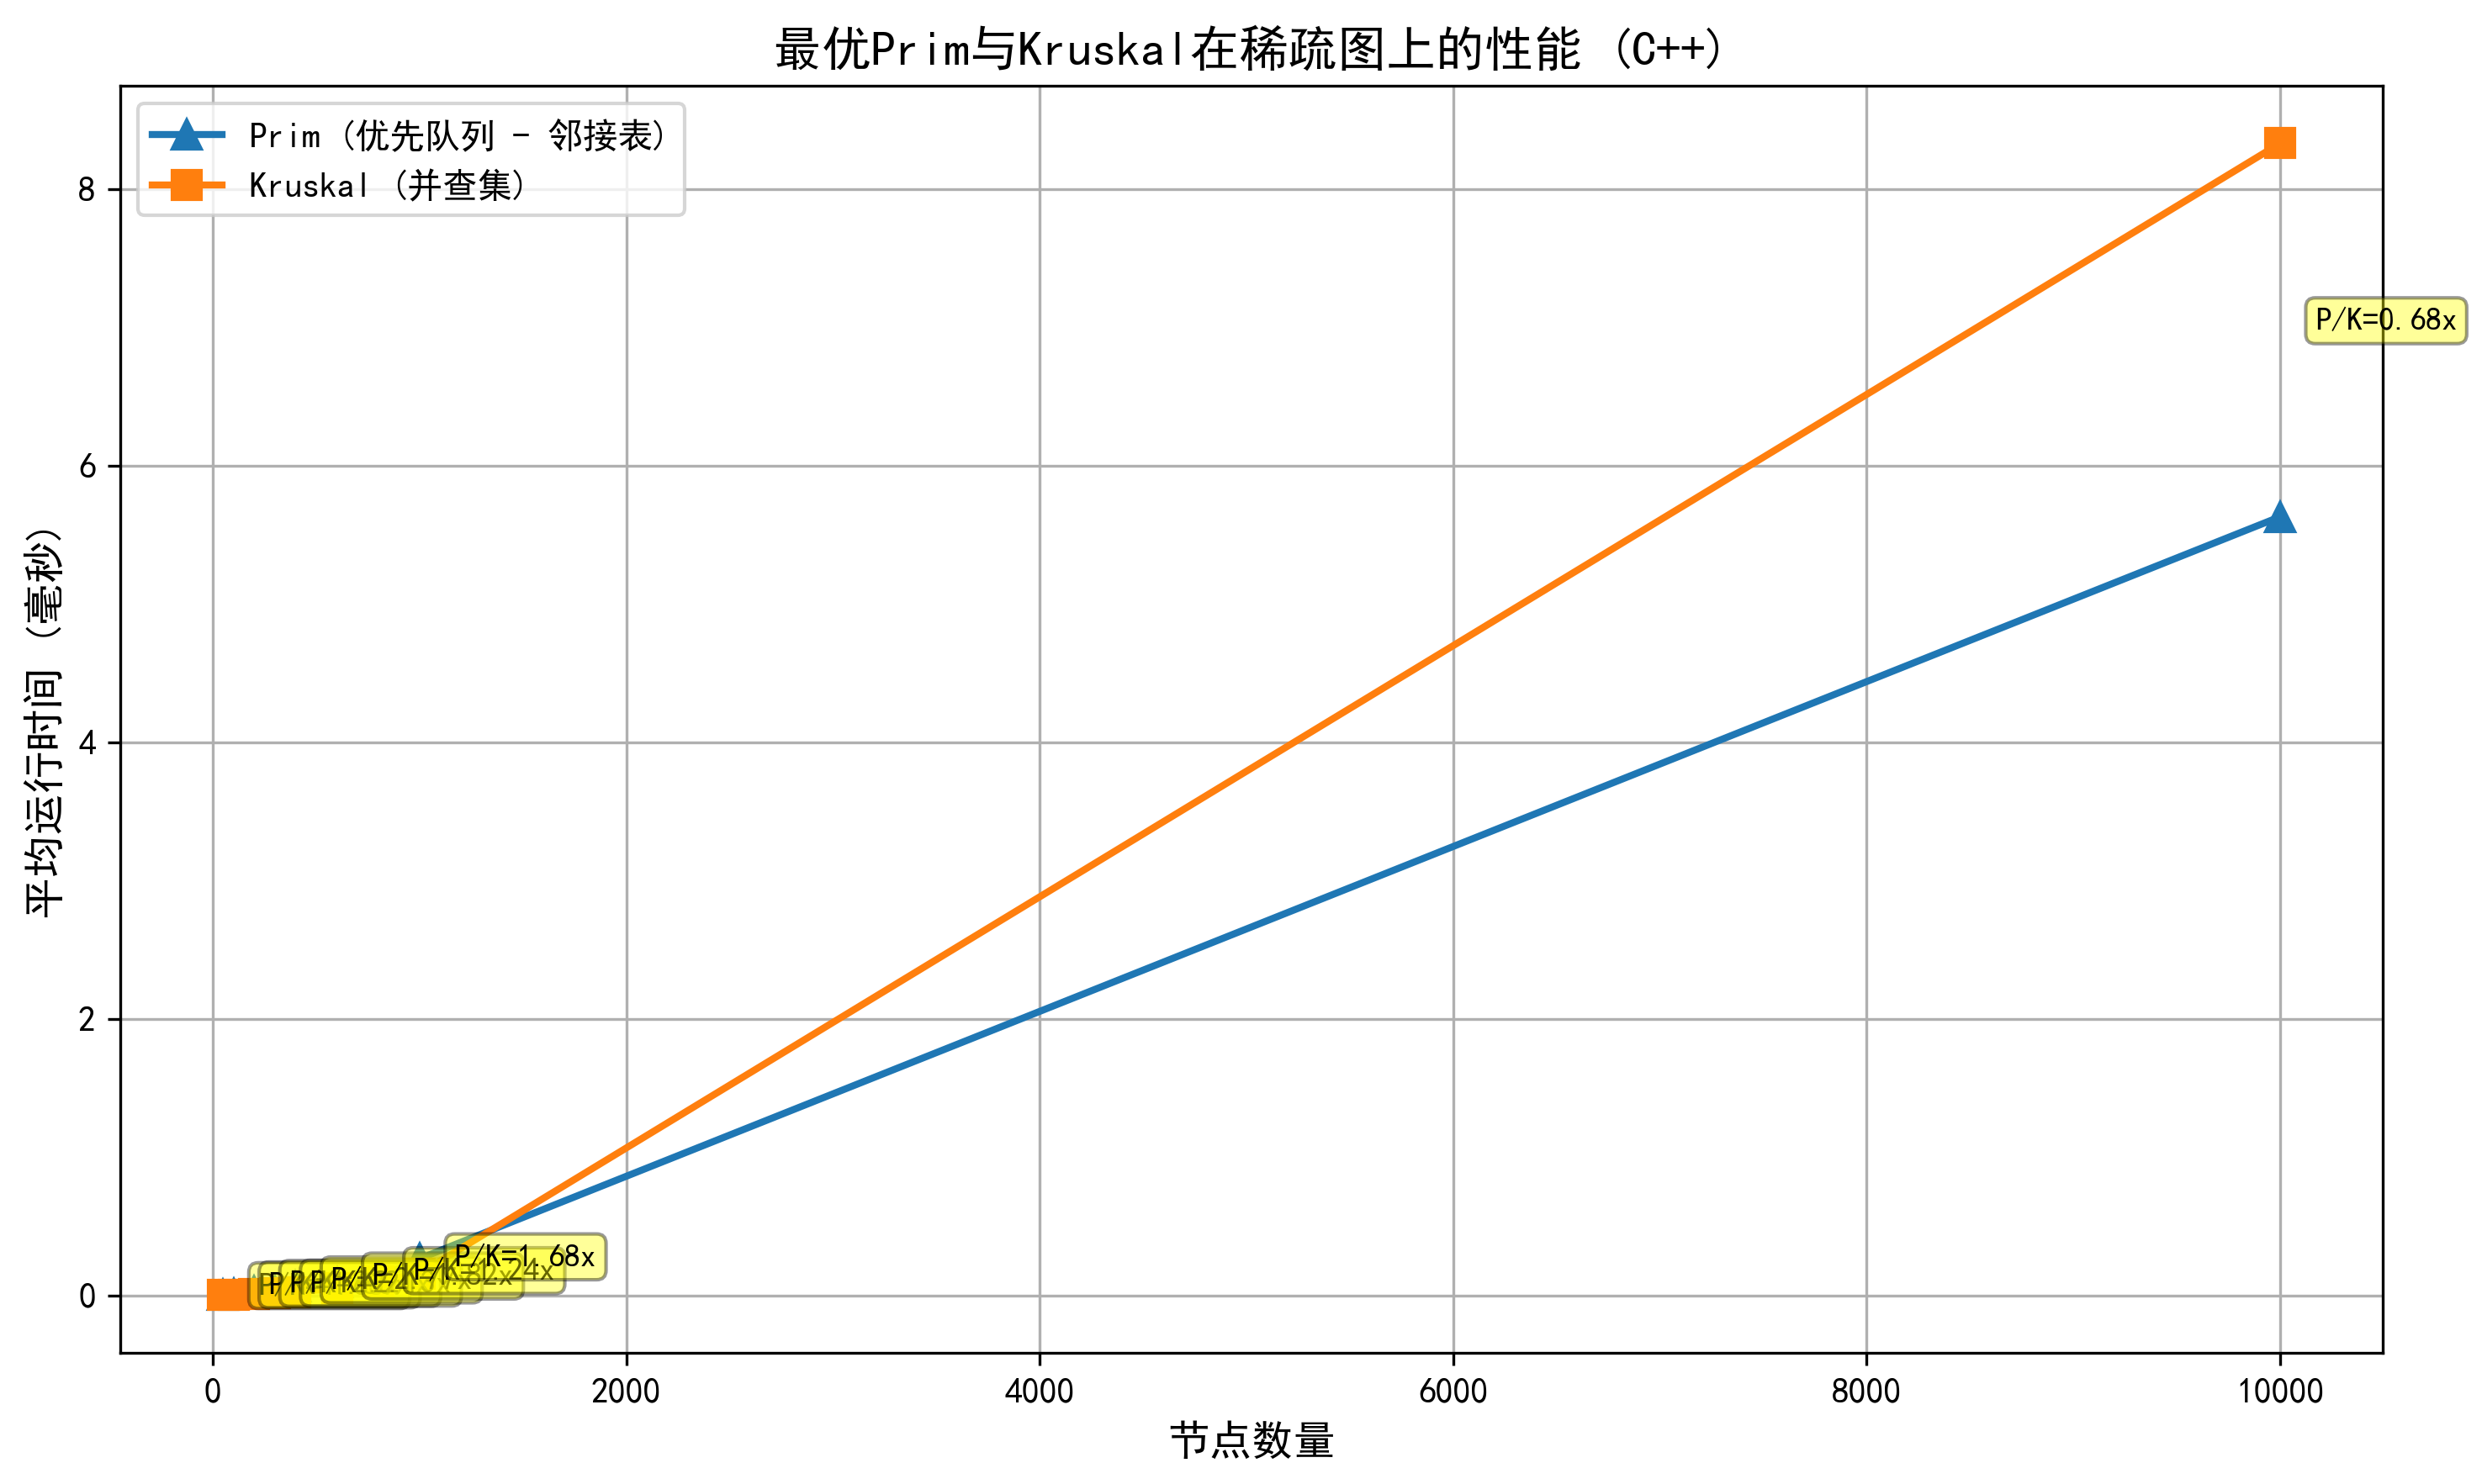
\includegraphics[width=0.8\textwidth]{img/img_cpp1/optimal_sparse_comparison_cpp.png}
    \caption{最优实现的Prim与Kruskal算法在稠密图上的性能比较}
    \label{fig:optimal_dense}
\end{figure}

\begin{figure}[htbp]
    \centering
    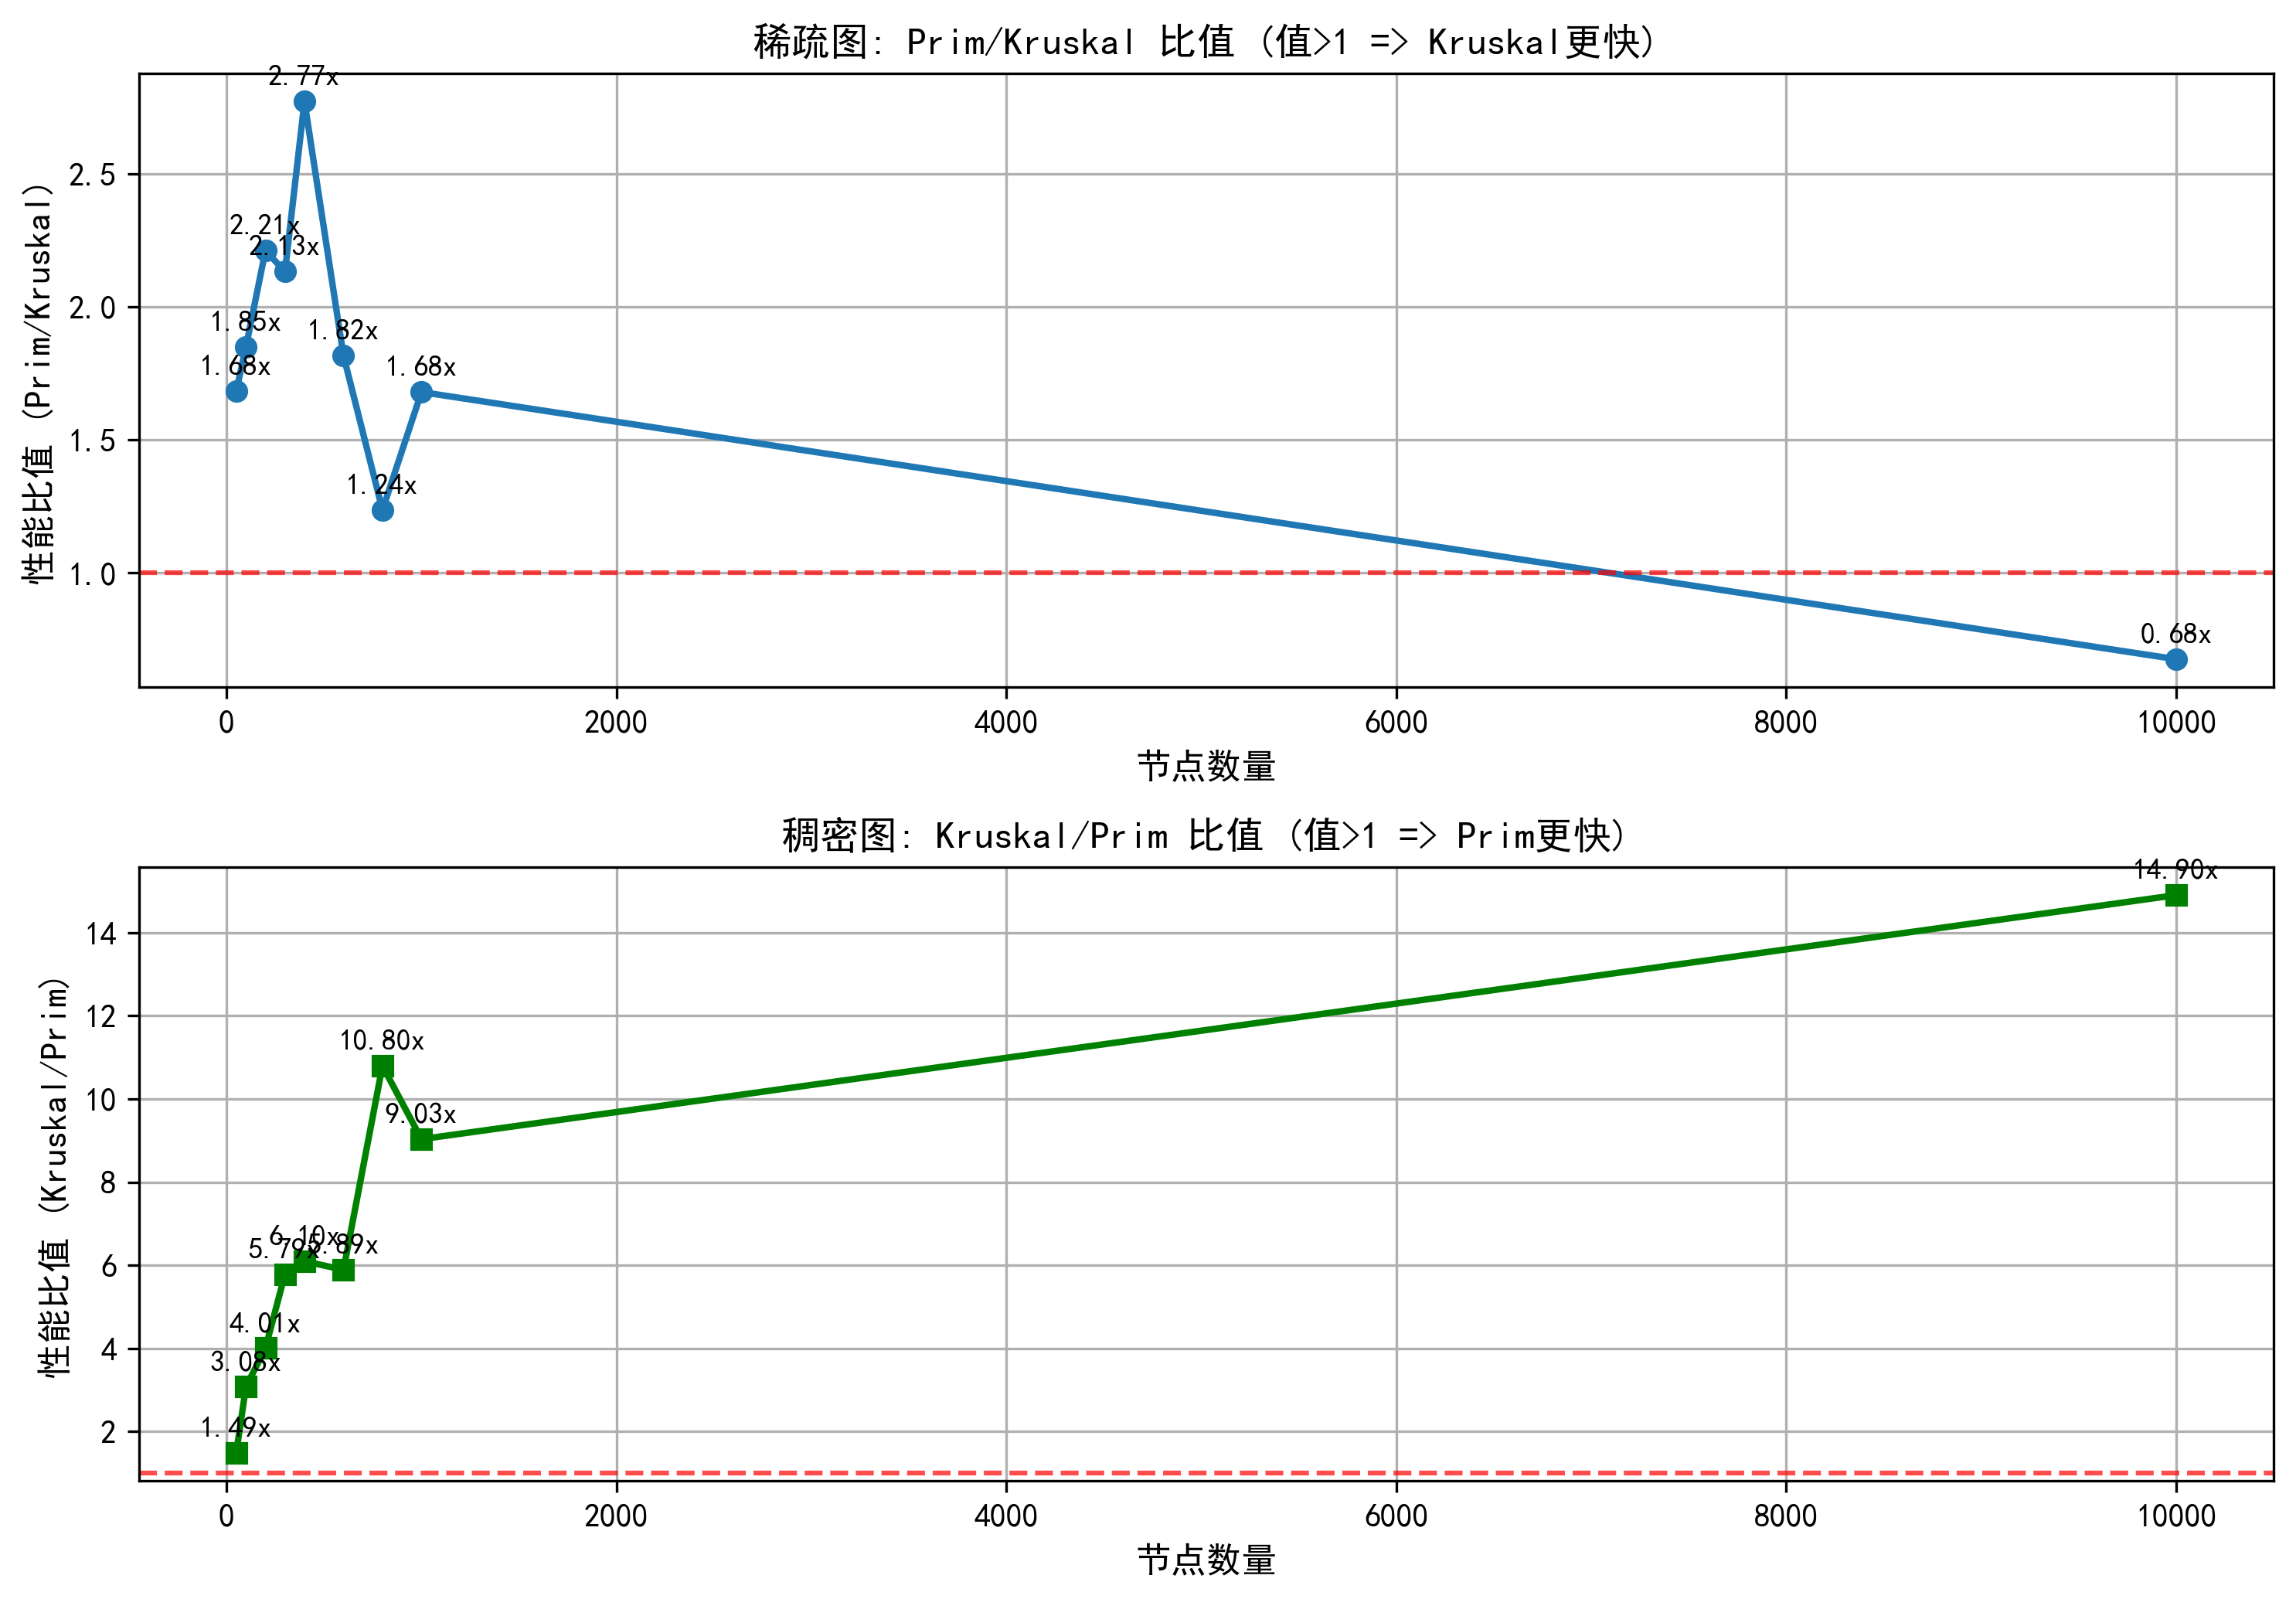
\includegraphics[width=0.8\textwidth]{img/img_cpp1/theory_vs_actual_cpp.png}
    \caption{最优实现的Prim与Kruskal算法性能比值}
    \label{fig:optimal_dense}
\end{figure}

原因可能推测如下:
\begin{itemize}
    \item \textbf{Kruskal算法的排序开销常数因子较大}: 即使理论复杂度相似,std::sort 对大量边进行排序的实际开销(包括比较和数据移动)可能比Prim算法中优先队列操作的累积开销要大。
    \item \textbf{内存访问局部性}: Prim算法(尤其使用邻接表时)通常具有更好的缓存局部性,缓存命中率更高,从而在实际运行中获得性能优势。而Kruskal算法的排序和并查集操作可能导致更多的缓存不命中。
    \item \textbf{图表示和边获取开销}: 如果Kruskal算法需要从邻接矩阵获取边(复杂度为O(V²)),这个预处理步骤在稠密图中会成为性能瓶颈,而Prim算法使用邻接表则可以避免这个问题。
\end{itemize}

\begin{itemize}
\item \textbf{与已有研究的比较}:
\begin{itemize}
    \item 我们的实验结果与Cormen等人\cite{cormen}的理论分析基本一致,但提供了更多关于实际性能的细节
    \item 与Sedgewick和Wayne\cite{sedgewick}的实验结果相比,我们的研究更加关注不同数据结构实现对算法性能的影响
    \item 我们的研究证实了在大规模图处理中,内存访问模式和缓存局部性的重要性\cite{cache_locality},这与现代计算机体系结构研究的趋势一致
\end{itemize}
\end{itemize}

\section{结论}
通过对Prim算法和Kruskal算法及其不同实现的实验分析,我们可以得出以下结论:

\begin{enumerate}
    \item \textbf{数据结构的选择对算法性能有显著影响}:
    \begin{itemize}
        \item Prim算法中,在稀疏图上优先队列+邻接表实现明显优于其他实现;在稠密图上三种实现差异相对较小
        \item Kruskal算法中,并查集实现在稀疏图上明显优于数组实现,但在稠密图上两种实现的性能差距较小,这主要是因为排序操作成为主导因素
    \end{itemize}
    
    \item \textbf{图的稠密程度对算法选择很重要}:
    \begin{itemize}
        \item 对于稀疏图(边数远小于顶点数的平方),并查集实现的Kruskal算法在小规模图上通常是最佳选择
        \item 对于稠密图(边数接近顶点数的平方),优先队列+邻接表实现的Prim算法明显表现更好
        \item 随着图规模增大,即使在稀疏图上,Prim算法的优势也会逐渐显现
    \end{itemize}
    
    \item \textbf{算法复杂度与实际性能}:
    \begin{itemize}
        \item 实际性能表现与理论时间复杂度基本一致
        \item 在大规模稠密图上,Kruskal算法的性能下降显著(高达7.4倍差距),与理论预期一致
        \item 在稀疏图上,Kruskal算法比Prim算法要快约1.3倍(节点数为500时)
        \item 常数因子和实现细节对算法性能有显著影响,尤其是排序操作和内存访问模式
    \end{itemize}
    
    \item \textbf{影响实际性能的关键因素}:
    \begin{itemize}
        \item \textbf{排序开销}:Kruskal算法在处理稠密图时,排序的常数因子开销较大,成为主导因素,掩盖了不同数据结构实现的差异
        \item \textbf{内存访问局部性}:Prim算法(特别是邻接表实现)通常具有更好的缓存局部性,这与现代计算机体系结构的特点相符\cite{cache_locality}。而Kruskal算法的排序和并查集操作可能导致更多的缓存不命中。
        \item \textbf{数据结构实现细节}:如优先队列中decrease-key操作的实现方式对Prim算法性能影响显著
        \item \textbf{图的表示方法}:预处理阶段从不同图表示中获取边的方式会影响总体性能
        \item \textbf{实际操作次数}:即使在稠密图中,MST的边数仍然只有 $V-1$ 条,限制了合并操作的实际执行次数
    \end{itemize}
    
    \item \textbf{实际应用建议}:
    \begin{itemize}
        \item 当处理小型稀疏图(如小规模道路网络)时,优先选择并查集实现的Kruskal算法
        \item 当处理大型稀疏图或任何规模的稠密图时,优先选择优先队列+邻接表实现的Prim算法
        \item 当图的规模较小时,可以选择实现简单的算法,因为性能差异不明显
        \item 在实际系统中,应考虑缓存友好性和内存局部性等因素,而不仅仅是理论复杂度
    \end{itemize}
\end{enumerate}

本实验使用C++实现了不同版本的最小生成树算法,并对其在不同图类型上的性能进行了比较。实验结果与理论分析基本一致,但也揭示了理论复杂度之外的实际性能影响因素。数据结构选择、图特性、内存访问模式和实现细节都对算法性能有重要影响。在实际应用中,应根据具体问题的图特性(规模和稠密程度)以及运行环境特点来选择合适的算法和实现方式,以达到最优的性能表现。

\begin{thebibliography}{9}
    \bibitem{ctex} CTEX.org, ``中文TeX排版系统'', 2023, \url{https://ctex.org/}
    
    \bibitem{cormen} Cormen, T. H., Leiserson, C. E., Rivest, R. L., \& Stein, C., ``Introduction to Algorithms'', MIT OpenCourseWare, 2009, \url{https://ocw.mit.edu/courses/6-046j-introduction-to-algorithms-sma-5503-fall-2005/}
    
    \bibitem{skiena} Skiena, S. S., ``The Algorithm Design Manual'', Algorithm Repository, 2020, \url{http://www3.cs.stonybrook.edu/~algorith/}
    
    \bibitem{sedgewick} Sedgewick, R., \& Wayne, K., ``Algorithms, 4th Edition'', Princeton University, 2022, \url{https://algs4.cs.princeton.edu/}
    
    \bibitem{boost} Boost C++ Libraries, ``Boost Graph Library: User Guide and Reference Manual'', 2022, \url{https://www.boost.org/doc/libs/1\_81\_0/libs/graph/doc/}
    
    \bibitem{cpp} Stroustrup, B., ``The C++ Programming Language'', ISO C++ Foundation, 2023, \url{https://isocpp.org/}
    
    \bibitem{mst_wiki} Wikipedia, ``Minimum spanning tree'', 2023, \url{https://en.wikipedia.org/wiki/Minimum\_spanning\_tree}
    
    \bibitem{prim_visual} Visualgo.net, ``Minimum Spanning Tree Visualizations'', 2023, \url{https://visualgo.net/en/mst}
    
    \bibitem{cache_locality} Drepper, U., ``What Every Programmer Should Know About Memory'', 2007, \url{https://people.freebsd.org/~lstewart/articles/cpumemory.pdf}
\end{thebibliography}
\end{document}